\documentclass[review]{elsarticle}

\usepackage{lineno,hyperref}
%\usepackage{lineno}
\modulolinenumbers[5]

\journal{Journal of Theoretical Computer Science}

%%%%%%%%%%%%%%%%%%%%%%%
%% Elsevier bibliography styles
%%%%%%%%%%%%%%%%%%%%%%%
%% To change the style, put a % in front of the second line of the current style and
%% remove the % from the second line of the style you would like to use.
%%%%%%%%%%%%%%%%%%%%%%%

%% Numbered
%\bibliographystyle{model1-num-names}

%% Numbered without titles
%\bibliographystyle{model1a-num-names}

%% Harvard
%\bibliographystyle{model2-names.bst}\biboptions{authoryear}

%% Vancouver numbered
%\usepackage{numcompress}\bibliographystyle{model3-num-names}

%% Vancouver name/year
%\usepackage{numcompress}\bibliographystyle{model4-names}\biboptions{authoryear}

%% APA style
%\bibliographystyle{model5-names}\biboptions{authoryear}

%% AMA style
%\usepackage{numcompress}\bibliographystyle{model6-num-names}
\usepackage{amsmath}
\usepackage{psfrag}
\usepackage{graphicx}
\usepackage{epsfig}
\usepackage{epstopdf}
\usepackage{amssymb}
\usepackage{bm}
\usepackage[dvipsnames]{xcolor}
\usepackage{mathtools}

%% `Elsevier LaTeX' style
\bibliographystyle{elsarticle-num}
%%%%%%%%%%%%%%%%%%%%%%%

\newcommand{\paral}{\; \vert \;}
\newcommand{\myvec}[1]{\overrightarrow{#1}}
\newcommand{\Defeq}{\stackrel{\mathrm{df}}{=}}
\newcommand{\Bnfeq}{::=}
\newcommand{\Co}[1]{\overline{#1}}

%
\newcommand{\Bsep}{\: \mid \: }
\newcommand{\Rule}[2]{\displaystyle{\frac{#1}{#2}}}
\newcommand{\SF}[1]{\mathsf{#1}}
\newcommand{\Act}{\mathsf{Act}}
\newcommand{\Vis}{\mathsf{Vis}}
\newcommand{\ActK}{\mathsf{ActK}}
\newcommand{\Proc}{\mathsf{Proc}}
\newcommand{\Procc}{\mathsf{ProcC}}
\newcommand{\Pred}{\mathsf{Pred}}
\newcommand{\Std}{\mathsf{Std}}
\newcommand{\rms}{\mathrm{S}}
\newcommand{\rmrec}{\mathrm{rec}}
\newcommand{\rmreck}{\mathrm{reck}}
\newcommand{\rmreckR}{\mathrm{reckR}}
\newcommand{\rma}{\mathrm{A}}
\newcommand{\rmp}{\mathrm{P}}
\newcommand{\rmf}{\mathrm{F}}
\newcommand{\rmr}{\mathrm{R}}
\newcommand{\rmfr}{\mathrm{FR}}
\newcommand{\equivS}{\equiv_{\mathrm{S}}}
\newcommand{\SigSA}{\Sigma_{\mathrm{SA}}}
\newcommand{\ltran}[1]{\stackrel{#1}{\longrightarrow}}
\newcommand{\tran}[1]{\stackrel{#1}{\rightarrow}}
\newcommand{\nottran}[1]{\stackrel{#1}{\not\rightarrow}}
\newcommand{\Rtran}[1]{\stackrel{#1}{\rightsquigarrow}}
\newcommand{\notRtran}[1]{\stackrel{#1}{\not\rightsquigarrow}}
\newcommand{\trans}[1]{\stackrel{#1}{\rightarrow}_{\mathrm{S}}}
\newcommand{\Par}{\mid}
\newcommand{\Mid}{\!\mid\!}
\newcommand{\restrict}[1]{\!\setminus\!#1}

\newcommand{\mA}{\mathcal{A}}
\newcommand{\mSA}{\mathcal{SA}}
\newcommand{\mWA}{\mathcal{WA}}
\newcommand{\mAK}{\mathcal{AK}}
\newcommand{\aAK}{\mathcal{(A)K}}
\newcommand{\umAK}{\underline{\mathcal{A}}\mathcal{K}}
\newcommand{\un}[1]{\underline {#1}}
\newcommand{\PI}{\mathcal{PI}}
\newcommand{\rom}[1]{\mbox{\rm{#1}}}

\newcommand{\Nil}{\mathbf{0}}
\newcommand{\New}[1]{\nu#1\: }
\newcommand{\Str}{\equiv}
\newcommand{\stdpred}{\mathsf{std}}
\newcommand{\std}[1]{\mathsf{std}(#1)}
%
\newcommand{\Bch}[2]{\mathsf{before}_{#1}(#2)}

\newcommand{\keys}[1]{\mathsf{keys}(#1)}
\newcommand{\kkey}[1]{\mathsf{k}(#1)}
\newcommand{\key}[1]{[#1]}
\newcommand{\Keys}{\mathcal{K}}
\newcommand{\freshpred}[1]{\mathsf{fsh}[#1]}
\newcommand{\fresh}[2]{\mathsf{fsh}[#1](#2)}

\newcommand{\ta}[1]{\mathsf{ta}(#1)}
\newcommand{\action}[1]{\mathsf{act}(#1)}

\newcommand{\intr}{\mbox{\ $\hat{}$\ }}
%\newcommand{\intr}{\mbox{\; $\widehat{}$\;}}
\newcommand{\sterm}{\mathsf{trm}}
\newcommand{\Sterm}[1]{\sterm(#1)}
\newcommand{\und}[1]{\underline{#1}}
\newcommand{\sqc}{\mathop{\cdot}}
\newcommand{\card}[1]{|#1|}
\newcommand{\bydef}{\stackrel{\emph{def}}{=}}
%
\newcommand{\Angle}[1]{\langle #1 \rangle}
\newcommand{\Tri}{\triangleright}
%\newcommand{\hole}{\bullet}
\newcommand{\hole}{[\ ]}
\newcommand{\rec}[1]{\mathrm{rec}\, #1}
\newcommand{\Rec}[1]{\rec #1 .}
\newcommand{\Rch}{\mathsf{Rch}}
\newcommand{\prune}{\pi}
\newcommand{\Prune}[1]{\prune(#1)}
\newcommand{\Root}[1]{\mathsf{rt}(#1)}

\newcommand{\Bis}{\sim}
\newcommand{\Biss}{\Bis_{\mathsf{S}}}
\newcommand{\Bisf}{\Bis_{\mathsf{F}}}
\newcommand{\Bisfr}{\Bis_{\mathsf{FR}}}
%\newcommand{\Bisu}{\Bis_{\Un}}
\newcommand{\Sim}{\mathcal{S}}
\newcommand{\Rem}{\backslash}
\newcommand{\sqeqt}{\sim}
% rules:
% static rule
\newcommand{\one}{\mbox{(I)}}
\newcommand{\onef}{\mbox{(1)}}
\newcommand{\oner}{\mbox{(1R)}}
% choice rule
\newcommand{\two}{\mbox{(II)}}
\newcommand{\twof}{\mbox{(2)}}
\newcommand{\twor}{\mbox{(2R)}}
% choice axiom
\newcommand{\thr}{\mbox{(III)}}
\newcommand{\thrf}{\mbox{(3)}}
\newcommand{\thrr}{\mbox{(3R)}}
\newcommand{\thrpf}{\mbox{(3\,$'$\!)}}
\newcommand{\thrpr}{\mbox{(3\,$'$\!R)}}
%
%
\newcommand{\Draft}[1]{}
\newcommand{\Comment}[1]{}
\newcommand{\Rev}[1]{{#1}^{-1}}
\newcommand{\rulename}[1]{\textsf{#1}}

\newcommand{\Blue}[1]{\textcolor{blue}{#1}}
%\newcommand{\Red}[1]{#1}
\newcommand{\Red}[1]{\textcolor{red}{#1}}
%
\newcommand{\DP}{\mathit{DP}}
\newcommand{\Me}{\mathit{Me}}
\newcommand{\Meprime}{\mathit{Me'}}
\newcommand{\MutS}{\mathit{MutS}}
\newcommand{\MutSprime}{\mathit{MutS'}}
\newcommand{\MutL}{\mathit{MutL}}
\newcommand{\MutH}{\mathit{MutH}}
\newcommand{\UvrD}{\mathit{UvrD}}
%

\newtheorem{theorem}{Theorem}
\newtheorem{definition}{Definition}
\newtheorem{remark}{Remark}
\newtheorem{example}{Example}
\newtheorem{proposition}{Proposition}
%
\newcommand{\xxrightarrow}{\xmapsto}

%

\begin{document}

\begin{frontmatter}

\title{Modelling of DNA Mismatch Repair with a reversible process calculus\tnoteref{mytitlenote}}
%\tnotetext[mytitlenote]{Fully documented templates are available in the elsarticle package on \href{http://www.ctan.org/tex-archive/macros/latex/contrib/elsarticle}{CTAN}.}

%% Group authors per affiliation:
\author{Stefan Kuhn}%\fnref{myfootnote}}
\address{School of Computer Science and Informatics, De Montfort University, Leicester, UK}
\ead{stefan.kuhn@dmu.ac.uk}
%\fntext[myfootnote]{Since 1880.}

\author{Irek Ulidowski}%\fnref{myfootnote}}
\address{School of Computing and Mathematical Sciences, University of Leicester, Leicester, UK}
\ead{iu3@leicester.ac.uk}

%\fntext[myfootnote]{Since 1880.}
%% or include affiliations in footnotes:
%\author[mymainaddress,mysecondaryaddress]{Elsevier Inc}
%\ead[url]{www.elsevier.com}

%\author[mysecondaryaddress]{Global Customer Service\corref{mycorrespondingauthor}}
%\cortext[mycorrespondingauthor]{Corresponding author}
%\ead{support@elsevier.com}
%
%\address[mymainaddress]{1600 John F Kennedy Boulevard, Philadelphia}
%\address[mysecondaryaddress]{360 Park Avenue South, New York}

\begin{abstract}
%We have demonstrated in previous work that the Calculus of Covalent Bonding (CCB) can be used to simulate higher-level biochemical processes. This is significant since CCB was originally devised to model organic chemical reactions on a lower level. We are now extending the use of CCB to model another gene repair pathway, DNA Mismatch Repair (MMR). This is a more complex pathway than the Base Excision Repair (BER) which we modelled originally. It involves four proteins and needs a distinction between the two chains in a DNA strand. We demonstrate that we can model this by extending our modelling of BER and that we can do this using the unchanged CCB calculus and operational semantics. We also show that the simulation software developed previously can be used to execute this pathway.
%
%
We have demonstrated in previous work that the Calculus of Covalent Bonding (CCB) can be used to simulate higher-level biochemical processes. This is significant since CCB was originally devised to model lower level organic chemical reactions. In this paper we extend the use of the calculus  to model an important gene repair pathway, namely DNA Mismatch Repair (MMR). This complex pathway involves four helper proteins and needs a distinction between the two chains in a DNA strand. 
In order to achieve this, we extend the calculus by allowing prefixing with collections of bonding sites.
% and its operational semantics by allowing more complex concerted actions transitions.
% We also show that the simulation software developed previously can be used to execute this pathway.
\end{abstract}

\begin{keyword}Reversible computation, Calculus of Covalent Bonding, DNA Mismatch Repair.
%\texttt{elsarticle.cls}\sep \LaTeX\sep Elsevier \sep template
%\MSC[2010] 00-01\sep  99-00
\end{keyword}

\end{frontmatter}

\linenumbers

\section{Introduction}

We have previously introduced a Calculus of Covalent  Bonding (CCB) \cite{KU16,KU2017} to models the formation and breaking of covalent bonds. % in organic molecules. 
CCB contains the possibility to link forming and breaking of bonds, thus enabling integrated, local control of reversibility. This feature allows us to represent both standard reversibility as well as \emph{out-of-causal order} reversibility~\cite{Irek2012}. In order to demonstrate the basics of our calculus we show how to model the autoprotlysis of water, which transfers a proton between two water molecules. 
%Since the reaction takes place in water it is also known as autoprotolysis of water. 
This reversible reaction is shown in Figure~\ref{fig:autoprotolysis}.
%
\begin{figure}
\centering
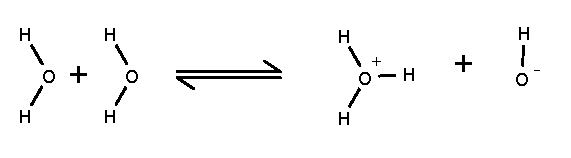
\includegraphics[height=2cm]{autoprotolysis}
\caption{Autoprotolysis of water.}
\label{fig:autoprotolysis}
\end{figure}

The main factor in the reaction is that oxygen is \emph{nucleophilic}, so it attracts electrons. This makes the hydrogen atoms in water
have a positive partial charge and the oxygen atoms a negative partial charge, attracting each other. Due to the nucleophilicity of 
oxygen, a covalent bond can form between them. This bond is formed out of electrons in the outer shell of the oxygen atom not used in bonds so far. Since a hydrogen atom cannot have more than one bond the creation of a new bond is compensated by breaking of the existing hydrogen-oxygen bond.
These reactions are \emph{concerted}, namely they happen together without a stable intermediate configuration. As a result we have reached the state where one oxygen has three covalent bonds to hydrogens and is positively charged,
and the other oxygen bonds to only one hydrogen and is negatively charged. The reaction is reversible: the oxygen, which has lost a hydrogen, can 
pull back one of the hydrogens from the other water.

We now outline the modelling of the reaction in CCB.  % to remind the reader of the basics of CCB. 
We model the hydrogen and oxygen atoms as processes $H$ and $O$ below, where 
$h,o$ are actions representing the bonding capabilities of the atoms and $n,p$ 
represent negative and positive charges respectively. $H',O'$ are process constants.
$$\begin{array}{lll}
H & \bydef & (h;p).H'\\
O & \bydef & (o,o,n).O'
\end{array}$$
We use a general prefixing construct $(s;b).P$ where $s$ is a sequence of actions or executed 
actions, and $b$ is a \emph{weak} action. Sometime the weak action is omitted 
(as in the definition of $O$). Informally, an action in $s$ can take place in any order, 
and $b$ can happen if
all actions in $s$ have already taken place. Once $b$ takes place, it must be accompanied by
undoing immediately one of the actions in $s$ (and thus possibly breaking a bond). We shall later extend
this prefixing operator to permit multiple bonding sites as in $((s;b)\mid \cdots\mid (s';b')).P$.

We use a synchronisation function $\gamma$ which tells us which actions can combine to 
produce bonds between atoms:
$$\begin{array}{lllllllllllllllll}
\gamma(h,o) = ho \quad &
\gamma(n,p) = np \quad &
\gamma(n,h) = nh\quad  &
\gamma(n,o) = no 
\end{array}$$
Each water molecule is a structure consisting of two hydrogen atoms and one oxygen atom 
which are bonded appropriately. 
$$( (h_1[1];p).H'_1 \paral (h_2[2];p).H'_2 \paral (o_1[1],o_2[2],n).O'_1)\setminus\{h_1,h_2,o_1,o_2\}$$
We have used subscripts to name the individual copies of 
atoms and actions. The system of two water molecules in Figure~\ref{fig:autoprotolysis} is represented 
by placing them in parallel and restricting actions $n$ and $p$. This is represented by  
the following process, where restrictions are moved outside using structural congruence laws:
\begin{flalign*}
& ( (h_1[1];p).H'_1 \paral (h_2[2];p).H'_2 \paral (o_1[1],o_2[2],n).O'_1 \paral \\ 
&\paral  (h_3[3];p).H'_3 \paral (h_4[4];p).H'_4  \paral (o_3[3],o_4[4],n).O'_2) 
\setminus\{h_3,h_4,o_3,o_4,h_1,h_2,o_1,o_2,n,p\}
\end{flalign*}
Now actions $n$ and $p$ of different water molecules can combine, representing a transfer of a proton from one atom 
of oxygen to another oxygen. We show below the transfer from $O_2$ to $O_1$, using the \emph{concerted actions} feature of CCB, where the actions to bond are indicated in bold blue and the bond to be broken is in bold red.
\begin{flalign*}
& ( (h_1[1];p).H'_1 \paral (h_2[2];p).H'_2 \paral (o_1[1],o_2[2],\Blue{\bm{n}}).O'_1 \paral 
(\Red{\bm{h_3[3]}};\Blue{\bm{p}}).H'_3 \\
&\paral (h_4[4];p).H'_4  \paral (\Red{\bm{o_3[3]}},o_4[4],n).O'_2) 
\setminus\{h_3,h_4,o_3,o_4,h_1,h_2,o_1,o_2,n,p\}\\
%
&\xrightarrow{\{ np[5], \underline{h_{3}o_{3}}[3]\}} \\
%
&( (h_1[1];p).H'_1 \paral (h_2[2];p).H'_2 \paral (o_1[1],o_2[2],\bm{n[5]}).O'_1 \paral 
(\bm{h_3};\bm{p[5]}).H'_3 \\
&\paral (h_4[4];p).H'_4  \paral (\bm{o_3},o_4[4],n).O'_2) 
\setminus\{h_3,h_4,o_3,o_4,h_1,h_2,o_1,o_2,n,p\}
\end{flalign*}

Since $H_3$ is weakly bonded to $O_1$ and its strong capability 
$h_3$ has become available, the bond $5$ gets promoted to a stronger bond, releasing 
the capability $p$ of $H_3$. This is done by the application of CCB's promotion rule:
\begin{flalign*}
\Rightarrow\; &( (h_1[1];p).H'_1 \paral (h_2[2];p).H'_2 \paral (o_1[1],o_2[2],n[5]).O'_1 \paral 
(h_3[5];p).H'_3 \\
&\paral (h_4[4];p).H'_4  \paral (o_3,o_4[4],n).O'_2) 
\setminus\{h_3,h_4,o_3,o_4,h_1,h_2,o_1,o_2,n,p\}
\end{flalign*}

We have now arrived at the state on the right hand side in Figure~\ref{fig:autoprotolysis}.
Oxygen $O_1$ is blocked, which represents it being fully bonded (and positively charged).
Oxygen  $O_2$ has a free $n$ capability and can abstract any of the hydrogens from $O_1$. 
As a result the process can reverse to its original state or to equivalent states where
different hydrogen atoms are bonded to $O_1$ and $O_2$.

In this paper, we model DNA mismatch repair using CCB. This builds upon and extends our previous work on the modelling of BER and other biochemical reactions~\cite{10.1007/978-3-319-99498-7_8}  and shows that the mechanisms in CCB are relevant outside its original application area. 

Deoxyribonucleic acid (DNA) carries the essential information for the working of all known organisms. It is composed of two polynucleotide chains. Each nucleotide contains one of the four nucleobases, or simply bases,  adenine (A), cytosine (C), guanine (G), and thymine (T). 
The bases can react with each other as follows: A and T produce a pair A-T, C and G produce a pair C-G,
and other combinations are not normally possible. This property means that each of the two polynucleotide chains of a DNA contains the same biological information, but expressed differently. It also enables DNA replication. 
DNA can split into two chains and then each chain can be completed with the matching bases, so that each new DNA is an identical copy of the original strand. Replication in turn enables the multiplication of cells and growth.

In reality DNA can be imperfect. This could be due either to external factors, such as radiation 
%(the reason why nuclear radition is damaging long-term) 
or internal factors, such as free radicals produced by the body. Another source of DNA errors are problems during replication. For example, it can happen that adenine in one chain faces guanine in the other chain when it should normally be matched by a thymine. Figure~\ref{fig:damages} shows such a mismatch on the right: The combination of the A/G bases is incorrect. Another error is an incorporation of a uracil base (U) in a DNA chain, which would normally not occur in DNA, is shown on the left in Figure~\ref{fig:damages}. A repair mechanism for this error, called Base Excision Repair (BER), was modelled in \cite{10.1007/978-3-319-99498-7_8} using our Calculus of Covalent Bonding (CCB).

\begin{figure}[h!]
  \centering
    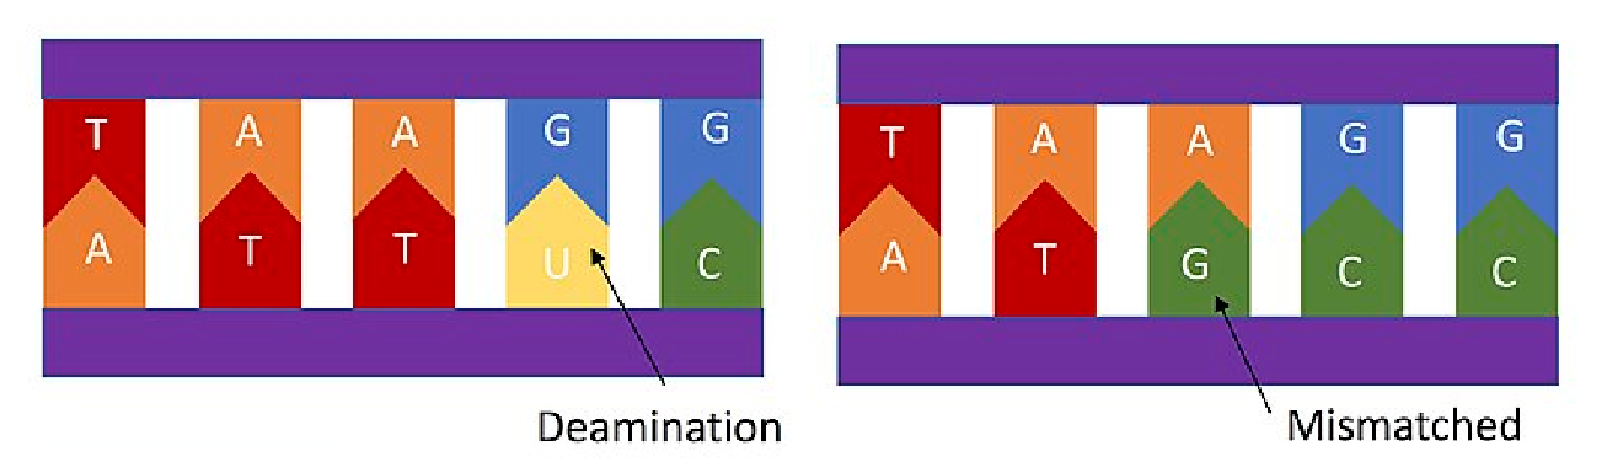
\includegraphics[width=1.0\textwidth]{Types_of_DNA_Damage_part}
  \caption[Two types of DNA damage.]{Two types of DNA damage. The right half shows a DNA mismatch.
  % (the example used here). 
  On the left, the incorporation of a Uracil base is shown.
  %, which was modelled in \cite{10.1007/978-3-319-99498-7_8}. 
  Part of \href{https://commons.wikimedia.org/wiki/File:Types_of_DNA_Damage.jpg}{Image} by Chantelmao, licensed under \href{https://creativecommons.org/licenses/by-sa/4.0/deed.en}{CC-BY-SA-4.0}.}
  \label{fig:damages}
\end{figure}

DNA repair is crucial to maintain the quality of information in organisms. Whilst DNA replication errors are rare (they happen at a rate of about 1 per every 100,000 nucleotides), this translates to a large number of errors given the length of DNA: about 120,000 mistakes every time a human cell divides~\cite{damage}. There are other sources of DNA damage, and also a multitude of repair mechanisms. We focus in this paper on a particular type of replication error called DNA Mismatch Repair (MMR) and its repair. Since incorrect DNA can give rise to cancer and other illnesses and generally to early ageing and death, DNA repair is a crucial part of life and its understanding is an important research topic.
%
We shall model around 30 molecules involved in the MMR system, and represent the reactions of the mechanism as transitions of the MMR system. On the one hand, this is a continuation of the biochemical modelling in our previous work and, on the other hand, it provides an opportunity to further test and evaluate CCB.  
A significant advantage of CCB is that it allows to represent out-of-causal order reversibility~\cite{Irek2012}, where causes are seemingly undone before their effects are undone, which is common in biochemical reactions.

%\Red{For modelling such situations, CCB is useful since it enables out-of-causal order reversibility. This is needed to model processes like the one on the rigtht in Figure~\ref{fig:introexample}. Here, a bond to one element (for example A) is needed when the bond to the nexte element (for example B) is formed to avoid losing the connection completely. Only once the new connection is formed, the old one can be released, which is out-of-causal order. A good modelling in a calculus requering causal consistency is not possible.}
%}

\section{Related Work}
This work has its origin in two strands of research. One of them is the simulation of chemical reactions and biological processes. The other one is research on process calculi to model computations. These have been merged  to better understand both areas of research.

In chemistry, speed of reactions and reactions rates have been modelled, with ordinary differential equations (ODEs) being an efficient tool \cite{higham}. Whilst such methods accurately show the dynamic behaviour, it was soon noted that they do not deal with the objects involved. In particular, any properties of the objects, which make reactions possible, are not considered. This became even more important when biochemical processes, which do not only involve small molecules, but also macromolecules, cells, and membranes, were modelled. This lack of understanding of the objects was raised in \cite{fontana} and the use of computer science methods like the $\lambda$-calculus was suggested.

A connection between process calculi and chemistry has been made in \cite{chamjournal}. Here, the Chemical Abstract Machine (CHAM) is introduced as a method to define the semantics of a calculus. As opposed to other semantics for calculi, the algebraic terms (“molecules”) can interact with each other no matter what order they are written in - this is similar to molecules being in a solution. CHAM also introduces membranes to group atoms and rules which simulate heating and cooling of solutions. The actual rules determining the reactions must be defined for a particular CHAM. Therefore, a CHAM can be used to execute processes of arbitrary process calculi. A CHAM can also model actual chemistry depending on the rules used. Starting with Regev et al. \cite{regev2000} process calculi, specifically the $\pi$-calculus, were used to model biochemical systems. An analogy between processes in concurrent computing and biological entities in natural systems, and between communication in computer systems and interactions between entities in biological systems is used for this. This is done by representing biological units as processes, their possible actions as channel ports and binding and unbinding as establishing and breaking a communication, respectively, on a channel. The stochastic $\pi$ calculus \cite{PriamiStochasticPi} was used to extend the model to include reaction rates \cite{PriameRegev}. This enables the simulation of the concentrations and of the overall state of the system over time.

Other work in the area include Bio-PEPA \cite{CiocchettaBiopepa}, which combines a process algebra with timing information and can represent reaction rates. In a Bio-PEPA simulation the entities modelled are species. Every interaction of molecules creates a new species, and there is no tracking of different “original” components. The transitions between the entities model the transformations between species. There is no tracking of mechanisms or modelling of the underlying causes. The focus is on the rates and the development of concentrations over time. P Systems \cite{psystems} was the first attempt to model membranes and compartments, with objects being able to move in and out of them. BioAmbients \cite{RegevBioambients} is based on the Ambient calculus [12], which was originally devised for mobile computing outside the biological context and is an extension of the $\pi$-calculus. Here, similarly to P systems, processes can be inside compartments (and compartments can be in other compartments as well). Brane Calculi (“brane” is short for membrane) \cite{CardelliMobileAmbients}, a family of process calculi, model membranes not only as compartments that define which interactions can happen, but as entities that can be transformed to gain new capabilities. Typical examples are viruses entering cells by interacting with their membranes. The Projective Brane Calculus \cite{ProjectiveBrane} is a variant where interactions are directed outward or inward from a membrane. Other formalims include the Language for Biochemical Systems (LBS) \cite{PlotkinLBS}, the Calculus of Chemical Systems \cite{PlotkinCCS}, and the Biochemical Abstract Machine (BIOCHAM) \cite{biocham}.

Modelling of biological processes using process algebras has been applied to various areas since the original publications. Apart from biochemical interactions (e.g
metabolic pathways [9], gene regulatory networks [62, 76], the cell-division cycle [10], inflammatory processes [68], RNA synthesis [16]), also processes involving organisms as entities were modelled, e.g. immune defence [42], epidemiology [114, 77], or ecological processes [111, 112, 113]. On the other hand, also the calculi used have been extended with new elements of syntax and associated rules for more realistic modelling of biological and chemical examples.
%
\section{A Calculus of Covalent Bonding}\label{sec:calculus}
%\section{Calculus of Covalent Bonding}\label{sec:calculus}
%
The Calculus of Covalent Bonding, or CCB for short, was defined in~\cite{KU2017}. 
We recall here the main definitions in order to make the paper self-contained. 
We note, however, that the syntax of this version of CCB is slightly extended, and a new `shortcut'  
SOS rule for three concerted actions is added. 
%Moreover, two new SOS rules for concerted actions are added. 
We first introduce some preliminary notions and notations.

Let $\mA$ be the set of (forward) action labels, 
ranged over by $a,b,c,d,e,f,h$ and $j$. We partition $\mA$ into the set of \emph{strong actions}, written as
$\mSA$, and the set of \emph{weak actions}, written as $\mWA$. 
%\textcolor{blue}{
Communication between pairs of actions model creating bonds and undoing such communications represents breaking bonds. Most bonds result from communication between strong actions, but some bonds also involve a weak action. When a bond involving a weak action is created it causes breaking a neighbouring bond on strong actions\footnote{Fuller explanation follows Definition~1 on page 16.
}
%}
Reverse (or past) action labels are members of
$\underline\mA$, with typical members $\un{a},\un b, \un c,\un d, \un e ,\un f, \un h$ and $\un j$, and represent 
undoing of actions. The set $\mathcal{P}(\mA \cup \underline\mA)$ is ranged over by $L$.

Let $\Keys$ be an infinite set of {\em communication keys} (or {\em keys} for short)
\cite{PhillipsUlidowski06,PHILLIPS200770}, ranged over by $k,l, m,n$. The Cartesian product $\mathcal A \times \Keys$, denoted by $\mAK$,
 represents past actions, which are written as $a[k]$ for $a\in \mA$ and $k\in\Keys$. 
Correspondingly, we have the set $\umAK$ that represents undoing of past actions. Letters $\alpha, \beta$ denote actions which are either from $\mA$ or $\mAK$. It will be 
useful to consider sequences of actions or past actions, namely the elements of $(\mA \cup \mAK)^*$, 
which are ranged over by $s,s'$, and sequences of purely past actions, namely the elements of $\mAK^*$, 
which are ranged over by $t,t'$. The empty sequence is denoted by $\epsilon$. We use ``$\alpha, s$'' and
``$s,s'$'' to denote a concatenation of elements, which can be strings or single actions.

We shall also use two sets of \emph{auxiliary action} labels, namely the set $(\mA) =\{ (a)\ \mid a\in\mA\}$, and its product with the set of keys, denoted by $(\mA)\Keys$. These labels will be used in the auxiliary rules when defining
the semantics of CCB.

Molecules may have several bonding \emph{sites} and several bonds can be created or dissolved at each bonding site. A site and its potential bonds are modelled via $(s;b)$, where $s$ is a sequence of actions, where actions model bonds, and $b$ is a weak (bond) action. The action $b$ can be omitted, in which case the construct is written as $(s)$. When a molecule has several sites 
$(s;b), \ldots,(s';b')$ we shall write them as $(s;b) \Mid  \ldots \Mid (s';b')$ by using the symbol ``$\paral$'' to indicate that sites bond independently of each other and that the order in which sites appear is irrelevant. Such expressions are called \emph{collections of sites}, or just collections, and will be used to define the prefix operator. More formally, a site $\sigma$
is either $(s;b)$ or $(s)$. A collection $\mu$ is either 
$\sigma$ or a composition of finitely many sites $\sigma\Mid\ldots\Mid \sigma$, where the order in which sites appear is irrelevant,
and $\epsilon$ is the empty collection of sites. We shall denote collections where all strong actions of all sites are fully bonded as $\eta$.


We now define the Calculus of Covalent Bonding. The syntax of CCB is given 
below where $P$ and $Q$ are process terms:
%$$P ::=  S \ \mid \ (s;b).P \ \mid \ P\paral Q \ \mid \ P\restrict L $$
$$P ::=  S \ \mid \ \mu.P \ \mid \ P\paral Q \ \mid \ P\restrict L $$
%
The set of process identifiers (constants) $\PI$ contains typical elements $S$ and $T$. 
A process identifier $S$ has normally a defining equation $S\bydef P$ where $P$ contains only forward 
actions (and no past actions). There is also a special identifier
 $\Nil$, denoting the deadlocked process, which has no defining equation.

We have a general prefixing operator $\mu.P$. This operator
extends the prefixing operators in \cite{DK2007}, \cite{Irek2012}, and {\cite{KU16,KU2017}. 
If each site of $\mu$ has only one action, then it is the multi-action prefix from \cite{DK2007}.
If the collection $\mu$ has only one site, then it is the general prefixing operator from \cite{KU16,KU2017}. 
If its only site has no weak action, then the prefixing is written as $(s).P$ and is called the
\emph{simple prefix}. 
The simple prefix is the prefixing operator in \cite{Irek2012}. 
One of the actions in $s$ in $(s).P$ may be a weak action from $\mWA$. If $s$ is a sequence that contains   
a single action, then the action is a strong action and the operator 
is the prefixing operator of CCS \cite{Milner1980}.
We omit trailing $\Nil$s so, for example, $(s).\Nil$ is written as $(s)$.
%
% Move this example to somewhere later
%
\Comment{\Stefan{We will only use cases in this paper where processes are of the form $(s).\Nil$. We still have the possibility of 
processes like $(s).(s').\Nil$ in our calculus. This could be used to model protein functions in biological systems, for example 
base excision repair (\cite{Koehler2014}. For this a protein ``walks'' along a strand of DNA and repairs faults which occurred in 
DNA replication. Such a protein could be modelled by having the walk modelled in $s$ and the repair mechanism in $s'$, combining them to a model like $(s).(s').\Nil$.}
}
%
%
An interesting feature of the operator $(s;b).P$ is the execution of the weak action $b$, which
can happen only after all the actions in $s$, which are strong actions, have taken place. Performing $b$ then forces
undoing one of the past actions in $s$ (by the \rulename{concert} rules in Figures~\ref{fig:c1sos}-\ref{fig:xc2sos}).

$P\paral Q$ represents two systems $P$ and $Q$ which can perform actions or reverse actions on
their own, or which can interact with each other according to a communication function
$\gamma$. As in the calculus ACP \cite{ACPBook}, the communication function is a partial function 
$\gamma: \mathcal A \times \mathcal A \rightarrow \mathcal A$ which is commutative and associative. The function
$\gamma$ is used in the operational semantics to define when two processes can interact. \Red{The use of a synchronization function instead of a $\tau$-style communication as in CCS was motivated in the original CCB by the potential bonding between many different atoms. This can easily be captured by desiging the atoms and the synchronizations separately.} Processes 
$P$ and $Q$ in $P\paral Q$ can also perform a pair of concerted actions,
which is a novel feature of our calculus.  We also have the ACP-like restriction operator 
$\setminus L$, where $L$ is a set of labels (subset of $\mathcal{P}(\mA \cup \underline\mA)$ ). 
%
It prevents actions from taking place and, due to 
the synchronisation algebra used, it also blocks communication. If $\gamma(a,b)=c$ then $a.P$ and $b.Q$
cannot communicate in $(a.P\paral b.Q)\setminus c$.
Note that we do not use here the usual relabelling 
operator $[f]$, where $f: \mA \rightarrow \mA$, which could be easily added.

%
%move this elsewhere?
%
\Comment{
The example in the Introduction and our main example in Section~\ref{sec:bigexample} seem to indicate that only
simple processes of the form $(s;b).\Nil$ are sufficient in the modelling of chemical reactions. 
However, there are examples where a nested prefix $(s;b).(s';b').P$ is useful. 
Consider a base excision repair as in \cite{Koehler2014} where a protein ``walks'' along 
a strand of DNA and repairs faults which occurred in the DNA replication. The walking along a DNA strand 
could be modelled by actions in $s$, and, once a fault is found, the repair mechanism could be modelled
by the actions in $s'$. Another example where the full calculus is useful is a model of long 
standing transactions with compensations in \cite{Irek2012}.
}

The set of \emph{process terms} is ranged over by $P$, $Q$ and $R$ and is denoted by $\Proc$. 
In the setting of CCB these terms are called \emph{processes}. 
A context $C\hole$ is a process term containing a \emph{hole}, represented by $\hole$. 
Formally, contexts are defined by the following syntax: 
$$C::= \hole\ \mid\ \mu.C\ \mid\  P\paral C \ \mid\  C \paral P \ \mid \ C\restrict L $$
The term $C[Q]$ denotes the result of filling the hole in the context $C\hole$ with $Q$.
%We say that $R$ is a \emph{subprocess} of $P$ if $P$ is $C[R]$ for some context $C\hole$.

We define the semantics of our calculus by a labelled transition system,
LTS for short, which is a structure $(St,L,\rightarrow: \subseteq St \times \mathit{Lab} \times St)$
with $St$ the set of states, $\mathit{Lab}$ the set of action labels and $\rightarrow: 
\subseteq St \times \mathit{Lab} \times St$ the labelled transition relation.
For CCB, the set of states $St$ is the set $\Proc$. 
%In practice, all our results and examples hold for \emph{consistent} processes, namely processes
%reachable from standard processes.
% (see Definition~\ref{consistent}). 
The action labels are the forward actions $\mAK$, 
the reverse actions $\umAK$ and the \emph{groups of concerted actions} $\mAK \times \umAK $. We shall
use $\omega$ to denote a typical action label.
%
%\cup  \mAK \times \umAK \times \umAK$. 
%
The labelled transition relation will be defined in terms of SOS rules (Figures~\ref{fig:fsos}--\ref{fig:sc}) 
and rewrite rules (Figure~\ref{fig:reduction}), where
the rules in Figures~\ref{fig:fsos}--\ref{fig:reversesos}
are influenced by \cite{Irek2007}.  
Note that sequences $s$ and $t$ in Figures~\ref{fig:fsos}--\ref{fig:xc2sos} 
are members of $(\mathcal{A}\cup\mathcal{AK})^*$ and $\mathcal{AK}^*$ respectively.

Next, we recall and explain the SOS rules before returning to 
the rewrite rules. Let $r$ be an SOS rule for an operator $f$ of CCB as in 
Figures~\ref{fig:fsos}--\ref{fig:sc}. 
%Then, $f$ is the operator of $r$ and the elements of $X$ are the arguments of $r$. 
%We write $rules(f)$ for the set of SOS rules for $f$. 
Transitions above the horizontal bar in $r$ are called \emph{premises}. 
The set of premises is written as
$pre(r)$. The transition below the bar in $r$ is the $\emph{conclusion}$ and 
is written as $con(r)$. 

%
\begin{figure}[t] 
\[
\begin{array}{ll}
\Rule
{}
{\std{\Nil}} \quad 
\Rule
{\std{P}}
{\std{S}}
\;\;
S \bydef P
\qquad &
\Rule
{}
{\fresh{m}{\Nil}} \quad
\Rule
{\fresh{m}{P}}
{\fresh{m}{S}}
\;\;
S \bydef P
\\[15pt]
%
\Rule
{\kkey{s}=\emptyset \quad  \std{P}}
{\std{(s;b).P}}
\qquad &
\Rule
{m \notin \kkey{s} \quad \fresh{m}{P}}
{\fresh{m}{(s;b).P}}
\\[15pt]
%
\Rule
{\kkey{s}=\emptyset \quad  \std{\mu.P}}
{\std{((s;b)\Mid \mu).P}}
\qquad &
\Rule
{m \notin \kkey{s} \quad \fresh{m}{\mu.P}}
{\fresh{m}{((s;b)\Mid \mu).P}}
\\[15pt]
%

\qquad &
\Rule
{m \notin \kkey{s} \quad m \neq n \quad \fresh{m}{P}}
{\fresh{m}{(s;b[n]).P}}
\\[15pt]
%
&
\Rule
{m \notin \kkey{s} \quad m \neq n \quad \fresh{m}{\mu.P}}
{\fresh{m}{((s;b[n])\Mid \mu).P}}
\\[15pt]
\Rule
{\std{P} \quad \std{Q}}
{\std{P \paral Q}}\quad 
\Rule
{\std{P}}
{\std{P \setminus L}}
\qquad &
\Rule
{\fresh{m}{P} \quad \fresh{m}{Q}}
{\fresh{m}{P \paral Q}}
\qquad 
\Rule
{\fresh{m}{P}}
{\fresh{m}{P \setminus L}}
\end{array}
\] 
\caption{Predicates $\mathsf{std}$ and $\mathsf{fsh}$.} 
\label{fig:predicates}
\end{figure}
%
%
We use two predicates $\std{P}:\Proc$ and $\fresh{m}{P}:\Keys \times \Proc$ in our SOS rules. 
They are defined in Figure~\ref{fig:predicates}, and they use two auxiliary functions
$\kkey{s}: (\mathcal{A}\cup\mathcal{AK})^* \rightarrow \mathcal{P}(\Keys)$ and
$\keys{P}: \Proc \rightarrow \mathcal{P}(\Keys)$. 
%
The function $\kkey{\_}$ is defined as follows:
$\kkey{\epsilon}=\emptyset$, $\kkey{\alpha:s}=\{l\}\cup\kkey{s} \text{ if }\alpha=a[l]$, for 
$a\in \mathcal{A}$ and $l\in \Keys$, and $\kkey{\alpha:s}= \kkey{s} \text{ if }\alpha \in \mathcal{A}$.
%
The function $\keys{\_}$ is given by $\keys{\Nil}=\emptyset$, $\keys{S}=\keys{P}$ if $S\bydef P$ and $S$ is guarded in $P$
(correspondingly for $\std{S}$ and $\fresh{m}{S}$ in Figure~\ref{fig:predicates}), 
$\keys{((s;\beta)\Mid \mu).P}=\kkey{s} \cup \kkey{\beta} \cup \keys{\mu.P}$, $\keys{P \paral Q}= \keys{P} \cup \keys{Q}$, and $\keys{P \restrict L}=\keys{P}$. Informally $\keys{P}$ associates with each term $P$ the set of its keys. 
A process $P$ is \emph{standard}, written $\std{P}$, if it contains no past actions (hence no keys). 
A key $n$ is \emph{fresh} in $Q$, written $\freshpred{n}(Q)$, if $Q$ contains no past action with the key $n$.
We extend the notion of fresh keys to the sequences of actions and past actions $s$ and $t$, and to sites $\sigma$, 
via the function $\kkey{\_}$. Moreover, correspondingly, $\freshpred{n}(\mu)$ if $\freshpred{n}(\sigma)$ for every
site $\sigma$ in $\mu$. 
%Figure~\ref{fig:predicates} defines the predicates by induction over the process terms. 
%We could also have said that $\std{P}$ is true if $\keys{P} = \emptyset$ and that 
%$\fresh{m}{P}$ is true if $i \notin \keys{P}$.

\begin{figure}[t] 
\[
\begin{array}{ll}
\rulename{s}\ 
\Rule
{\fresh{k}{s,s'}}
{(s,a,s';b) \xrightarrow{a[k]}_s (s,a[k],s';b)}
\qquad &
\rulename{c}\
\Rule
{\sigma \xrightarrow{a[k]}_s \sigma'\quad \fresh{k}{\mu}}
{\sigma \paral \mu \xrightarrow{a[k]}_s \sigma' \paral \mu}
%
\\[25pt]
\rulename{act1}\ 
\Rule
{\std{P} %\quad \fresh{k}{\mu}
   \quad \mu \xrightarrow{a[k]}_s \mu'}
{\mu.P \xrightarrow{a[k]}\mu'.P}
\qquad &
\rulename{act2}\
\Rule
{P \xrightarrow{a[k]} P' \quad \fresh{k}{\eta}}
{\eta.P \xrightarrow{a[k]} \eta.P'}
\\[25pt]
%\rom{act3}\ Dec 17
%\Rule
%{\std{P} \quad \fresh{k}{t,t'}}
%{(t,b,t';b').P \xrightarrow{b[k]}(t,b[k],t';b').P}
%\qquad &
%\\[25pt]
\rulename{par}\
\Rule
{P \xrightarrow{a[k]} P'\quad \fresh{k}{Q}}
{P \paral Q \xrightarrow{a[k]} P' \paral Q}
\qquad &
\rulename{com}\
\Rule
{P \xrightarrow{a[k]} P' \quad Q \xrightarrow{d[k]} Q'}
{P \paral Q \xrightarrow{c[k]} P' \paral Q'}
%\; (*)
%
\\[25pt]
\rulename{res}\
\Rule
{P \xrightarrow{a[k]} P'}
{P\backslash L \xrightarrow{a[k]} P'\backslash L}
\; a \notin L
\qquad &
\rulename{con}\
\Rule
{P \xrightarrow{a[k]} P'}
{S \xrightarrow{a[k]} P'}
\; S \bydef P
\end{array}
\] 
\caption{Forward SOS rules. We assume $\gamma(a,d)=c$.% and $b \in \mathcal{WA}$.
} 
% caption at submission \caption{Forward SOS rules. The condition (*) is $\gamma(a,d)=c$, and $b \in \mathcal{WA}$.} 
\label{fig:fsos}
\end{figure}

\begin{example}
{\rm
We illustrate how processes compute forwards using the new prefixing operator. Initially, we consider processes where collections have single sites only. Consider a standard
process $(a;b).(c) \paral (a,d,c)$ and the communication function $\gamma$ given by $\gamma(a,a)=a$ 
and $\gamma(c,c)=c$. We have
$$(a;b).(c) \paral  (a,d,c) \xrightarrow{a[1]} (a[1];b).(c) \paral  (a[1],d,c)$$
by the SOS rules \rulename{act1} and \rulename{com} from Figure~\ref{fig:fsos}. This is because $(c)$ 
is standard and the key 1 is fresh in $\varepsilon$. The next step of computation involves a communication of
the actions $c$, which we obtain by rules \rulename{act2} and \rulename{com}:
$$(a[1];b).(c) \paral  (a[1],d,c) \xrightarrow{c[2]} (a[1];b).(c[2]) \paral  (a[1],d,c[2])$$
We note that the key 2 is fresh in $a[1]$. Finally, the action $d$ takes place by \rulename{act1} and,
informally, the symmetric version of \rulename{par}.
$$(a[1];b).(c[2]) \paral  (a[1],d,c[2]) \xrightarrow{d[3]} (a[1];b).(c[2]) \paral  (a[1],d[3],c[2])$$
Formally, we use \rulename{par}, the structural congruence rule \rulename{sc} in Figure~\ref{fig:sc}
and the reduction rule \rulename{red1} in Figure~\ref{fig:reduction}.
}
\end{example}

\begin{figure}[t]
\[
\begin{array}{ll}
\rulename{rev s}\ 
\Rule
{
%\fresh{k}{s,s'}
}
{(s,a[k],s';\beta) \xrightarrow{\underline{a}[k]}_s (s,a,s';\beta)}
\qquad &
\rulename{rev c}\
\Rule
{\sigma \xrightarrow{\underline{a}[k]}_s \sigma'\quad \fresh{k}{\mu}}
{\sigma \paral \mu \xrightarrow{\underline{a}[k]}_s \sigma' \paral \mu}
\\[25pt]
%
\rulename{rev act1}\
\Rule
{\std{P} %\quad \fresh{k}{s,s'}
\quad \mu \xrightarrow{\underline{a}[k]}_s \mu' }
{\mu.P \xrightarrow{\underline{a}[k]}\mu'.P}
\quad &
%
% b was previously beta. Since we must apply prom rewrite before we apply any SOS rule, we do not 
% need a rule with a beta.
%
% referees suggested to remove fsh predicates from both act rules. They were there for symmetry reason 
% with the forward rules but are not used in the reverse.
%
\rulename{rev act2}\
\Rule
{P \xrightarrow{\underline{a}[k]} P' %\quad \fresh{k}{t}
}
{\eta.P \xrightarrow{\underline{a}[k]} \eta.P'}
\\[25pt]
% Dec 17
%\rom{rev act3}\
%\Rule
%{\std{P}  \quad \fresh{k}{t,t'} }
%{(t,b[k],t';b').P \xrightarrow{\underline{b}[k]} (t,b,t';b').P'}
%& \\[25pt]
\rulename{rev par}\
\Rule
{P \xrightarrow{\underline{a}[k]} P'\quad \fresh{k}{Q}}
{P \paral Q \xrightarrow{\underline{a}[k]} P' \paral Q}
\quad &
\rulename{rev com}\
\Rule
{P \xrightarrow{\underline{a}[k]} P' \quad Q \xrightarrow{\underline{d}[k]} Q'}
{P \paral Q \xrightarrow{\underline{c}[k]} P' \paral Q'}
%\; (*)
%
\\[25pt]
\rulename{rev res}\
\Rule
{P \xrightarrow{\underline{a}[k]} P'}
{P\backslash L \xrightarrow{\underline{a}[k]} P'\backslash L}
\; a \notin L
\quad &
\rulename{rev con}\
\Rule
{P \xrightarrow{\underline{a}[k]} P'}
{P \xrightarrow{\underline{a}[k]} S}
\; S \bydef P'
\end{array}
\]
\caption{Reverse SOS rules. We assume $\gamma(a,d)=c$, and 
and $\beta$ is either $b$ or $b[l]$ for $b \in \mathcal{WA}$. %Note that $\beta \in \mA \cup \mAK$.
} 
% at submission \caption{Reverse SOS rules. The condition (*) is $\gamma(a,d)=c$, and 
%and $\beta$ is either $b$ or $b[l]$ for $b \in \mathcal{WA}$.
%} 
\label{fig:reversesos}
\end{figure}

\begin{figure}[t] 
$$
\begin{array}{l}
\rulename{w}\
\Rule
{\fresh{l}{t}}
{(t;b) \xrightarrow{(b)[l]}_s (t;b[l])} \qquad\qquad
\rulename{cw}\
\Rule
{\sigma \xrightarrow{(b)[l]}_s \sigma'\quad \fresh{l}{\mu}}
{\sigma \paral \mu \xrightarrow{(b)[l]}_s \sigma' \paral \mu}
\\[20pt]
\rulename{aux1}\ 
\Rule{\std{P} % \quad \fresh{k}{t}
  \quad \mu\xrightarrow{(b)[k]}_s \mu'}
{\mu.P \xrightarrow{(b)[k]}\mu'.P}
\qquad
\rulename{aux2}\
\Rule
{P \xrightarrow{(b)[k]} P' \quad \fresh{k}{\eta}}
{\eta.P \xrightarrow{(b)[k]} \eta.P'}
\\[25pt]
\rulename{concert2'}\ 
\Rule
{P\xrightarrow{(b)[k]} P'\xrightarrow{\underline{a}[l]}P'' \qquad Q\xrightarrow{\alpha[k]}Q'\xrightarrow{\underline{d}[l]}Q''% %\quad \fresh{k}{Q} 
 }
{P \paral Q\xrightarrow{\{e[k],\underline{f}[l]\}} P'' \paral Q''}\\[25pt]
\rulename{concert2}\ 
\Rule
{U\equiv P \paral Q \quad  P\xrightarrow{(b)[k]}P'\xrightarrow{\underline{a}[l]}P'' 
  \quad Q\xrightarrow{\alpha[k]}Q' 
  \quad R\xrightarrow{\underline{d}[l]}R'% %\quad \fresh{k}{Q} 
 }
{U \paral R\xrightarrow{\{e[k],\underline{f}[l]\}} P'' \paral Q'\paral R'} \\[25pt]
%\rulename{concert3}\ 
%\Rule
%{U\equiv P \paral Q \quad  P\xrightarrow{(b)[k]}P'\xrightarrow{\underline{a}[l]}P'' 
%  \quad Q\xrightarrow{\alpha[k]}Q' \xrightarrow{\underline{g}[m]}Q''
 % \quad R\xrightarrow{\underline{d}[l],\underline{h}[m]}R'' % %\quad \fresh{k}{Q} 
 %}
%{U \paral R\xrightarrow{\{e[k],\underline{f}[l]\},\underline{j}[m]} P'' \paral Q''\paral R''}\\[25pt]

\end{array}$$
\caption{SOS rules for two concerted actions transitions. We assume $\alpha$ is $c$ or $(c)$ 
and $\gamma(b,c)=e$ for some $c\in \mathcal{A}$, $\gamma(a,d)=f$, and  $\gamma(g,h)=j$. The symbol `$\equiv$' 
denotes syntactic congruence. Additionally, we assume that actions $(b)[k]$ and $\underline{a}[l]$ in \rulename{concert2'} 
and \rulename{concert2} occur in the same site of $P$ and correspondingly for $(c)[k]$, $\underline{d}[l]$ and $Q$ 
in \rulename{concert2'}.}
\label{fig:c1sos}
\end{figure}


\begin{figure}[t] 
\[
\begin{array}{l}
\rulename{concert act}\
\Rule
{P \xrightarrow{\{{a}[k], \underline{h}[l]\}} P' \quad \fresh{k}{\eta}}
{\eta.P \xrightarrow{\{{a}[k], \underline{h}[l]\}} \eta.P'}\\[25pt]
%\rulename{concert3 act}\
%\Rule
%{P \xrightarrow{\{{a}[k], \underline{h}[l], \underline{j}[m]\}} P' \quad \fresh{k}{\eta}}
%{\eta.P \xrightarrow{\{{a}[k], \underline{h}[l], \underline{j}[m]\}} \eta.P'}\\[25pt]
\rulename{concert2 par}\
\Rule
{P \xrightarrow{\{{a}[k], \underline{h}[l]\}} P'\quad \fresh{k}{Q} \quad \fresh{l}{Q}}
{P \paral Q \xrightarrow{\{{a}[k], \underline{h}[l]\}} P' \paral Q}\\[25pt]
%\rulename{concert3 par}\
%\Rule
%{P \xrightarrow{\{{a}[k], \underline{h}[l], \underline{j}[m]\}} P'\quad \fresh{k}{Q} \quad \fresh{l}{Q}\quad \fresh{m}{Q}}
%{P \paral Q \xrightarrow{\{{a}[k], \underline{h}[l], \underline{j}[m]\}} P' \paral Q}\\[25pt]
\rulename{concert2 res}\
\Rule
{P \xrightarrow{\{{a}[k], \underline{h}[l]\}} P'}
{P\backslash L \xrightarrow{\{{a}[k], \underline{h}[l]\}} P'\backslash L}\;\;  a, \underline{h}  \notin L \cup (L)\\[25pt]
%\rulename{concert3 res}\
%\Rule
%{P \xrightarrow{\{{a}[k], \underline{h}[l], \underline{j}[m]\}} P'}
%{P\backslash L \xrightarrow{\{{a}[k], \underline{h}[l], \underline{j}[m]\}} P'\backslash L}\;\;  a, \underline{h}, \underline{j}  \notin L \cup (L)
%
\end{array}
\] 
\caption{SOS rules for the prefix, parallel composition and restriction and concerted transitions.
\label{fig:xc2sos} 
}
\end{figure}

\Comment{
\begin{figure}[t] 
\[
\begin{array}{l}
\rulename{concert3}\ 
\Rule
{U\equiv P \paral Q \quad  P\xrightarrow{(b)[k]}P'\xrightarrow{\underline{a}[l]}P'' 
  \quad Q\xrightarrow{\alpha[k]}Q' \xrightarrow{\underline{g}[m]}Q''
  \quad R\xrightarrow{\underline{d}[l]} R'\xrightarrow{\underline{h}[m]}R'' % %\quad \fresh{k}{Q} 
 }
{U \paral R\xrightarrow{\{e[k],\underline{f}[l]\},\underline{j}[m]} P'' \paral Q''\paral R''}\\[25pt]
%\rulename{concert2 act}\
%\Rule
%{P \xrightarrow{\{{a}[k], \underline{h}[l]\}} P' \quad \fresh{k}{\eta}}
%{\eta.P \xrightarrow{\{{a}[k], \underline{h}[l]\}} \eta.P'}\\[25pt]
\rulename{concert3 act}\
\Rule
{P \xrightarrow{\{{a}[k], \underline{h}[l], \underline{j}[m]\}} P' \quad \fresh{k}{\eta}}
{\eta.P \xrightarrow{\{{a}[k], \underline{h}[l], \underline{j}[m]\}} \eta.P'}\\[25pt]
%\rulename{concert2 par}\
%\Rule
%{P \xrightarrow{\{{a}[k], \underline{h}[l]\}} P'\quad \fresh{k}{Q} \quad \fresh{l}{Q}}
%{P \paral Q \xrightarrow{\{{a}[k], \underline{h}[l]\}} P' \paral Q}\\[25pt]
\rulename{concert3 par}\
\Rule
{P \xrightarrow{\{{a}[k], \underline{h}[l], \underline{j}[m]\}} P'\quad \fresh{k}{Q} \quad \fresh{l}{Q}\quad \fresh{m}{Q}}
{P \paral Q \xrightarrow{\{{a}[k], \underline{h}[l], \underline{j}[m]\}} P' \paral Q}\\[25pt]
%\rulename{concert2 res}\
%\Rule
%{P \xrightarrow{\{{a}[k], \underline{h}[l]\}} P'}
%{P\backslash L \xrightarrow{\{{a}[k], \underline{h}[l]\}} P'\backslash L}\;\;  a, \underline{h}  \notin L \cup (L)\\[25pt]
\rulename{concert3 res}\
\Rule
{P \xrightarrow{\{{a}[k], \underline{h}[l], \underline{j}[m]\}} P'}
{P\backslash L \xrightarrow{\{{a}[k], \underline{h}[l], \underline{j}[m]\}} P'\backslash L}\;\;  a, \underline{h}, \underline{j}  \notin L \cup (L)
%
\end{array}
\] 
\caption{Shortcut SOS rules for the three concerted actions transitions.  We assume $\alpha$ is $c$ or $(c)$ 
and $\gamma(b,c)=e$ for some $c\in \mathcal{A}$, $\gamma(a,d)=f$, and  $\gamma(g,h)=j$.
\label{fig:xc3sos} 
}
\end{figure}
}

\begin{figure}[t] 
\[
\begin{array}{l}
%\rom{sc}\
\Rule
{P \Rightarrow Q \quad Q \tran{\omega} Q' \quad Q' \Rightarrow P'}
{P\tran{\omega} P'} 
%\quad \mu \in \mAK\cup \umAK \cup \mathcal{C}
%%TODO Moreover, $S\equiv P$ for all $S, P$ 
%%such that $S\bydef P$.
\end{array}
\] 
\caption{Structural congruence rule \rulename{sc} when $\omega \in \mAK \cup (\mAK\times \umAK)$
% \cup  (\mAK\times \umAK\times \umAK))$,
and \rulename{rev sc} when $\omega \in \umAK$.} 
\label{fig:sc}
\end{figure}

\begin{figure}[t] 
\[
\begin{array}{lll}
\rulename{red1}: & P\Par Q \Rightarrow Q\Par P& 
\\[2pt]
\rulename{red2}: & P\Par (Q\Par R) \Rightarrow (P\Par Q)\Par R &
\\[2pt]
\rulename{red3}: & (P\Par Q)\Par R \Rightarrow P\Par (Q\Par R) & 
\\[2pt]
\rulename{red4}: & P\Par \Nil \Rightarrow P & 
\\[2pt]
\rulename{red5}: & (P\paral Q)\backslash L \Rightarrow P\backslash L \paral Q & \mbox{ if fn(Q)} \cap L = \emptyset
\\[2pt]
\rulename{red6}: & P\backslash L \paral Q \Rightarrow (P\paral Q)\backslash L & \mbox{ if fn(Q)} \cap L = \emptyset
\\[2pt]
\rulename{prom}: & ( (s,a,s';b[k])\mid \mu).P \Rightarrow ((s,a[k],s';b)\mid \mu).P & \mbox{ if } a \in \mathcal{SA}, b \in \mathcal{WA} 
\\[2pt]
\rulename{move}: & ((s,a,s',b[k],s'')\mid \mu).P \Rightarrow ((s,a[k],s',b,s'')\mid \mu).P & \mbox{ if } a \in \mathcal{SA}, b \in \mathcal{WA}
%\rulename{move-r}: & ((s,a,s',b[k],s'')\mid \mu).P \Rightarrow ((s,a[k],s',b,s'')\mid \mu).P & \mbox{ if } a \in \mathcal{SA}, b \in \mathcal{WA}
%\\[2pt]
%\rulename{move-l}: & ((s,b[k],s',a,s'')\mid \mu).P \Rightarrow ((s,b,s',a[k],s'')\mid \mu).P & \mbox{ if } a \in \mathcal{SA}, b \in \mathcal{WA}
\end{array}
\] 
\caption{Reduction rules. Sequences $s, s', s''$ are members of $(\mathcal{A} \cup \mathcal{AK})^{*}$.} 
\label{fig:reduction}
\end{figure}

The next example illustrates how some of the reverse SOS rules work. We only consider here processes with collections that consist of single sites. 
\begin{example}
{\rm 
Consider $(a[1],b).(c).S$ where $S\bydef (a,b).(c).S$. We have 
$$(a[1],b).(c).S \xrightarrow{\underline{a}[1]} (a,b).(c).S$$ by \rulename{rev act1} since $(c).S$ is standard.
Since $(a,b).(c).S$ is the definition of $S$ we obtain by rule \rulename{rev con} $(a[1],b).(c).S \xrightarrow{\underline{a}[1]} S$.
}
\end{example}

Figures  \ref{fig:fsos}--\ref{fig:reversesos} contain the usual SOS rules that define single action transitions of CCB. An auxiliary transition relation $\xrightarrow{}_s$ is used there to define operational changes to sites and collections of sites.  


Figures \ref{fig:c1sos}--\ref{fig:xc2sos} contain the SOS rules that define the novel concerted actions transitions. 
The main rules are the \rulename{concert} rules in Figure~\ref{fig:c1sos} that define when a pair %or a triple 
of concerted actions take place. 
We also have there four auxiliary rules \rulename{w}, \rulename{cw}, \rulename{aux1} and \rulename{aux2} which 
define only an auxiliary action transition relation needed in the \rulename{concert} rules.
Note that transitions in \rulename{aux1} and \rulename{aux2} use the auxiliary labels $(b)[k]$ 
for all $b \in \mWA$ and $k \in \Keys$. Also note that the three \rulename{concert} rules use \emph{lookahead} \cite{Uli92}.



The rules \rulename{concert par} in Figure~\ref{fig:xc2sos} require that $k$ is fresh in $Q$,
correspondingly as in \rulename{par}. Moreover, we need to ensure that when we reverse $h$ with the key $l$
in $P$ we do not leave out any actions with the key $l$ in $Q$ which make up a multi-action 
communication with the key $l$. Hence, we also include the premise $\fresh{l}{Q}$ in \rulename{concert par} rules. Correspondingly for the key $m$ in $Q$.
The two rules \rulename{concert act} require, correspondingly as \rulename{act}, that $k$ is fresh in $t$.
Our operational semantics guarantees that if a standard process evolves to $(t;b).P$, where all actions in $t$ are fully executed, and
$P$ reverses an action with the key $l$, then $l$ is fresh in $t$. Hence, we do not include $\fresh{l}{t}$
in the premises of the \rulename{concert act} rules.

We now illustrate how concerted actions transitions work.

\begin{example}\label{ex:examp1}
{\rm Consider the process $(a;b) \paral a \paral d$ with $\gamma(a,a)=c$ and $\gamma(b,d)=f$. After the
initial synchronisation of actions $a$, which produces the transition $c[1]$, we can bond weak $b$ with strong $d$ producing $f$, and at the same time break the $c$ bond. This is represented by a transition
with a pair of concerted actions:
$$(a[1];b) \paral a[1] \paral  d \xrightarrow{\{f[2], \underline{c}[1]\}} 
  (a;b[2])\paral a \paral d[2]$$
The transition is derived by rule \rulename{concert2} in Figure~\ref{fig:c1sos}
 since $(a[1];b) \xrightarrow{(b)[2]} (a[1];b[2]) \xrightarrow{\underline{a}[1]} (a;b[2])$ by \rulename{aux1} and \rulename{rev act1}, 
and since $a[1] \paral d \xrightarrow{f[2]} a[1] \paral d[2] \xrightarrow{\underline{a}[1]} a \paral d[2]$
by \rulename{par} and \rulename{rev par}.}
\end{example}
%
The next example illustrates a creation of a bond between weak actions.
\begin{example}\label{ex:examp2}
{\rm Consider $(a[1];b)\paral (a[1];b)$ with $\gamma(a,a)=c$ and $\gamma(b,b)=d$. Recall that actions $b$ here are weak.
We have the following pair of concerted actions derived by \rulename{concert2'}, where the bond created and the bond broken are between the same two processes:
 $$(a[1];b)\paral (a[1];b)  \xrightarrow{\{d[2], \underline{c}[1]\}} 
(a;b[2])\paral (a;b[2])\ . $$
This transition cannot be derived by \rulename{concert2} because we only have two processes here and \rulename{concert2} requires at least three separate processes. Note that \rulename{concert2'} can be used to derive  
  $$(a[1];b)\paral (a[1], b)  \xrightarrow{\{d[2], \underline{c}[1]\}} (a;b[2])\paral (a, b[2])\ . $$
 }
\end{example}

%
%
\Comment{There are situations where creation of a bond between weak actions of two processes requires breaking of bonds with other processes. %Such transitions cannot be derived by \rulename{concert1}, so we use other concert rules in Figure~\ref{fig:c1sos}.

\begin{example}\label{ex:concert3}
{\rm Consider $(a[1];b)\paral (e[2];b)\paral (a[1],e[2])$ with $\gamma(a,a)=c$, $\gamma(b,b)=d$, and
$\gamma(e,e)=h$.
The process cannot perform any concerted actions by \rulename{concert2'}: Although $(a[1];b)  \xrightarrow{(b)[l]} 
\xrightarrow{\underline{a}[1]} (a;b[l])$, for any $l$ different from 1 and 2, but
$(e[2];b)\paral (a[1],e[2])$  cannot perform the auxiliary $(b[l])$
transition since there are no SOS rules for parallel composition and auxiliary actions $(b)$. This forces us
to treat $(a[1];b)$ and $ (e[2];b)$ as $P$ and $Q$ in \rulename{concert2'}, respectively, and we notice that
we cannot undo a communication on $a$ or $e$. However, this is precisely what \rulename{concert2} allows, so we have these two different concerted actions transitions:
$$
(a[1];b)\paral (e[2];b)\paral (a[1],e[2])  \xrightarrow{\{d[3], \underline{c}[1]\}} 
(a;b[3])\paral (e[2];b[3])\paral (a,e[2])
$$ 
$$
(a[1];b)\paral (e[2];b)\paral (a[1],e[2])  \xrightarrow{\{d[3], \underline{h}[2]\}} 
(a[1];b[3])\paral (e;b[3])\paral (a[1],e)
$$ 
We notice that, following the first transition above, the $h[2]$ bond can be broken, and correspondingly the $c[1]$ bond can be broken after the second transition:
$$
(a;b[3])\paral (e[2];b[3])\paral (a,e[2]) \xrightarrow{\underline{h}[2]}  (a;b[3])\paral (e;b[3])\paral (a,e)
$$ 
$$
(a[1];b[3])\paral (e;b[3])\paral (a[1],e)  \xrightarrow{\underline{c}[1]} (a;b[3])\paral (e;b[3])\paral (a,e) 
$$ 
Creation of the $d[3]$ bonds makes the $h[2]$ and $c[1]$ bonds unstable, so they break immediately
after the corresponding concerted actions. Since creation and breaking of such bonds is almost instantaneous, we are using
a ``shortcut'' SOS rule to captures such cascade of two concerted actions and a reversal of an unstable action, called \rulename{concert3}. It allows us to derive
$$
(a[1];b)\paral (e[2];b)\paral (a[1],e[2])  \xrightarrow{\{d[3], \underline{c}[1], \underline{h}[2]\}} 
(a;b[3])\paral (e;b[3])\paral (a,e) .
$$ 
Here, creation of the bond $d$ results in two other bonds $c, h$ being broken. The rule \rulename{concert3} and the related rules
are in Figure~\ref{fig:xc3sos}.}
\end{example}
}


Overall, the transitions in Figures~\ref{fig:fsos}--\ref{fig:sc} are labelled with $a[k] \in \mAK$, or with 
$\underline{c}[l] \in \umAK$, or with concerted actions $(a[k], \underline{c}[l])$.
%  or $(a[k], \underline{c}[l], \underline{e}[m])$.
%\} \in \mathcal{C}$.

We also have the usual structural congruence rules 
\rulename{sc} and \rulename{rev sc} in Figure~\ref{fig:sc}, 
which potentially combine reductions (defined below) with transitions.

Next, we introduce our reduction relation which is given by the reduction (rewrite) rules 
in Figure~\ref{fig:reduction}. The reduction relation is needed to define {\em promotion} 
of actions. First we define {\em free names} of processes. 
%
%\begin{definition} \normalfont 
The function 
$\mathsf{fn}: \Proc \rightarrow \mathcal{P}(\Keys)$ is given as follows: 
$\mathsf{fn}(\Nil) = \emptyset$,
$\mathsf{fn}(S)=\mathsf{fn}(P) \text{ if }  S\bydef P$, 
$\mathsf{fn}((\sigma\mid \mu).P)=\mathsf{f}(\sigma)\cup \mathsf{fn}(\mu.P)$, where $\mathsf{f}(\sigma)$ is the set of all action labels in $\sigma$,
$\mathsf{fn}(\varepsilon.P)=\mathsf{fn}(P) $, $\mathsf{fn}(P\paral Q)=\mathsf{fn}(P) \cup \mathsf{fn}(Q)$, and $\mathsf{fn}(P \restrict L)=\mathsf{fn}(P) \restrict L$.
%\end{definition}


The reduction rules have names such as, for example, \rulename{red} and we write 
\rulename{red}: $P \Rightarrow Q$
to indicate that the reduction rule $P \Rightarrow Q$ is called \rulename{red}. 
The process $P$ in the rule
$P\Rightarrow Q$ is called a \emph{redex}, and the process $Q$ is called a \emph{contractum}. 
A reduction rule $P\Rightarrow Q$ can be seen as a prescription 
for deriving rewrites $C[P] \Rightarrow C[Q]$ for arbitrary context $C[\ ]$. 
A $P$ redex may be replaced by its contractum $Q$ in an arbitrary context 
$C[\ ]$ giving rise to a reduction step: $C[P] \Rightarrow C[Q]$.

\begin{definition} \normalfont The reduction relation $\Rightarrow$ is the smallest reflexive and 
transitive relation on CCB processes that is preserved by all contexts, and that satisfies the rules 
in Figure~\ref{fig:reduction}.
\end{definition}
Note that we do not want $\Rightarrow$ to be symmetric as we wish to apply \rulename{prom} and \rulename{move} only 
from left to right. 

The rewrite rules in Figure~\ref{fig:reduction} include 
\rulename{prom} and \rulename{move}
%, and \rulename{move-l} 
which promote weak bonds (here $b$) to strong bonds (here $a$). Recall that the order of actions in $s$ in expressions for sites
$(s)$ and $(s;b)$ is irrelevant.
The rule \rulename{prom} applies to the full version of site expression (with the ; construct), and
\rulename{move} applies only to the simple site expressions without `;'.
These two rules model what happens in chemical systems: a bond on a weak action is 
temporary and as soon as there is a strong action that can accommodate that bond (as the result
of concerted actions) the bond establishes itself on the strong action thus releasing the weak action.
In order to align the use of these two rules to what happens in chemical reactions, we insist
that they are used as soon as they becomes applicable: this is made 
precise in Definition~\ref{LTS}.
%We could have used the idea of ordering on SOS rules and rewrite rules \cite{irek2002,mousavi}
%to specify that the rewrite rules \rulename{prom}, \rulename{move-r} and \rulename{move-r} are higher 
%in the ordering than all SOS rules and the remaining rewrite rules, implying that they should 
%be applied first when deriving transitions. Alternatively, we could have tried to 
%employ some of the techniques presented in \cite{Cleaveland2001711} to define our transition relation.
%This would require the use of negative information in the premisses, and the definitions in the style
%as those in \cite{irek2002,mousavi}.  However, since we combine SOS rules
%with rewrite rules, we opted for a directly defined transition relation.

We now define the transition relation for the labelled transition system for CCB.
Recall that the states of the LTS are processes in $\Proc$ and the labels are members of $\mA$,
$\mAK$, $\aAK$ and the concerted actions labels in $\mAK \times \umAK$.
%or $\mAK \times \umAK \times \umAK$. 
First, the transition relation on collections sites, $\rightarrow_s$, 
is defined as the smallest relation derived by the rules \rulename{s}, \rulename{c},  \rulename{rev s}, \rulename{rev c},   
\rulename{w}, and \rulename{cw} in Figures~\ref{fig:fsos}--\ref{fig:c1sos}.  Second, the transition relation $\rightarrow$ is defined
as the smallest relation derived by the rules in Figures~\ref{fig:fsos}--\ref{fig:sc}. 
%
In order to define our transition relation $\mapsto$ we introduce processes in \emph{normal forms}: $\mathsf{nf}(P)$ is the set of $P'$ 
such that $P\Rightarrow P'$ and $P'$ cannot be reduced via \rulename{prom} or  \rulename{move}.



\begin{definition}\label{LTS} \normalfont
We associate to $\Proc$ and $\mAK \cup \umAK \cup \aAK \cup (\mAK \times \umAK) $
a transition relation $\mapsto$ given by $P \xmapsto{\omega} Q$ if $P \xrightarrow{\omega} P'$ for some $P'$ and $Q \in \mathsf{nf}(P')$. 
\end{definition}



\Comment{
Let $d:\Proc \rightarrow \mathbb{N}$ be the operator depth function defined by 
$d(P)=0$ if $P$ is a constant, and $d(f(P_1,\ldots,P_n))=1+max\{d(P_i)\vert 1 \leq i \leq n\}$ 
otherwise, where $f$ is an operator of CCB. The transition relation is given as follows:
%
%
\begin{definition}\label{LTS} \normalfont
We associate to $\Proc$ and $\mAK \cup \umAK \cup \aAK \cup (\mAK \times \umAK) 
\cup (\mAK \times \umAK\times \umAK) $
a transition relation
$\rightarrow$ given by $ \bigcup_{l<\omega} \rightarrow^l$, where transition relations
$\rightarrow^l \subseteq \Proc \times ( \mAK \cup \umAK \cup \aAK \cup (\mAK \times \umAK) \times 
 (\mAK \times \umAK\times \umAK)) \times  \Proc$
are as follows, with $b\in \mAK$ and $\mu \in \mAK \cup \umAK \cup (\mAK \times \umAK)
\cup (\mAK \times \umAK\times \umAK) $:

\begin{enumerate}
\item
$P \xrightarrow{(b)[k]} P' \in \rightarrow^l$ if $d(P)=l$,
$P \xrightarrow{(b)[k]} P'= con(r)$, where $r$ is either \rulename{aux1} or \rulename{aux2},
and each premise in $pre(r)$ is a valid transition in $\bigcup_{k<l} \rightarrow^k$, a valid transition $\rightarrow_s$, 
 or a valid predicate.

\item $P \tran{\mu} P'\in \rightarrow^l$ if $d(P)=l$, $P\Rightarrow Q$, for some $Q$ such that $Q$
does not contain any \rulename{prom}, \rulename{move-r} and \rulename{move-l} redex,  $Q \tran{\mu} Q'= con(r)$,
for some rule $r$ where each member of $pre(r)$ is either a valid transition
in $ \bigcup_{k<l} \rightarrow^k$, a valid transition $\rightarrow_s$, a valid rewrite or a valid predicate, and $Q'\Rightarrow P'$.

\end{enumerate}

\end{definition}

The first part of the definition specifies the auxiliary transitions using rules \rulename{aux1} and 
\rulename{aux2}. The second
part tells us how to use the remaining rules to define transitions. If $P$ has no \rulename{prom}, 
\rulename{move-r} and \rulename{move-l} redex, then we apply our rules in a standard way. Otherwise, we are 
required to reduce $P$ to $Q$ with \rulename{prom}, \rulename{move-r} and \rulename{move-l} first, 
then we define a transition of $Q$ to $Q'$
in a standard way, and finally we reduce $Q'$ to $P'$ (if needed). This implies that 
if $P$ has a \rulename{prom}, \rulename{move-r} or \rulename{move-l} redex, then we must use one 
of the structural congruence rules in Figure \ref{fig:sc}. 
And, if we use any of these rules, then the reduced process $Q$ must no longer have any 
\rulename{prom}, \rulename{move-r} and \rulename{move-l} redex. 
%A different way to define our transition 
%could be to employ some of the techniques suggested in \cite{Cleaveland2001711}
%that employ SOS rules with predicates. This would require the use of negative information in the premisses, 
%so we opted for the alternative approach which is based on the orderings on SOS rules and rewrite rules. 
}
%
\Comment{
\Stefan{Our approach for prioritising transitions is different from approaches using predicates in the premises of the SOS rules, as 
suggested for example in \cite{Cleaveland2001711}. In our case we decided for a different approach since we need to prioritise rewrite rules as well as SOS rules.}
}

The next example illustrates the application of the promotion rewrite rule.
\begin{example}\label{example4}
{\rm The transition 
$(a[1];b) \paral a[1] \paral  b \xrightarrow{\{d[2], \underline{c}[1]\}} (a;b[2])\paral a \paral b[2]$ 
from Example \ref{ex:examp1} cannot give rise to the corresponding $\mapsto$ transition which is followed by a communication of actions $a$. This is because there
is a \rulename{prom} redex $(a;b[2])$ in $(a;b[2])\paral a \paral b[2]$. The rewrite of this redex takes 
priority: the bond 2 moves from the weak $b$ to the strong $a$ by \rulename{prom}. Since 
$(a;b[2])\paral a \paral b[2] \Rightarrow (a[2];b)\paral a \paral b[2] $ and the contractum cannot be reduced with \rulename{prom} or
with \rulename{move}, we have 
$$(a[1];b) \paral a[1] \paral  b \xmapsto{\{d[2], \underline{c}[1]\}} (a[2];b)\paral a \paral b[2]$$

As a result, we can bond on the weak $b$ again and, importantly, the $a[2]$ to $b[2]$ bond is irreversible
as $\gamma(a,b)$ is undefined. Note that reaching
this bond by computing forwards alone is not possible.}
\end{example}

There are situations where creation of a bond between weak actions of two processes requires breaking of bonds with other processes. %Such transitions cannot be derived by \rulename{concert1}, so we use other concert rules in Figure~\ref{fig:c1sos}.

\begin{example}\label{ex:concert3}
{\rm Consider $(a[1];b)\paral (e[2];b)\paral (a[1],e[2])$ with $\gamma(a,a)=c$, $\gamma(b,b)=d$, and
$\gamma(e,e)=h$.
The process cannot perform any concerted actions by \rulename{concert2'}: Although $(a[1];b)  \xrightarrow{(b)[l]} 
\xrightarrow{\underline{a}[1]} (a;b[l])$, for any $l$ different from 1 and 2, but
$(e[2];b)\paral (a[1],e[2])$  cannot perform the auxiliary $(b[l])$
transition since there are no SOS rules for parallel composition and auxiliary actions $(b)$. This forces us
to treat $(a[1];b)$ and $ (e[2];b)$ as $P$ and $Q$ in \rulename{concert2'}, respectively, and we notice that
we cannot undo a communication on $a$ or $e$. However, this is precisely what \rulename{concert2} allows, so we have these two different concerted actions transitions:
$$
(a[1];b)\paral (e[2];b)\paral (a[1],e[2])  \xrightarrow{\{d[3], \underline{c}[1]\}} 
(a;b[3])\paral (e[2];b[3])\paral (a,e[2])
$$ 
$$
(a[1];b)\paral (e[2];b)\paral (a[1],e[2])  \xrightarrow{\{d[3], \underline{h}[2]\}} 
(a[1];b[3])\paral (e;b[3])\paral (a[1],e)
$$ 
Promotion can be applied in both cases giving us the transitions
$$
(a[1];b)\paral (e[2];b)\paral (a[1],e[2])  \xmapsto{\{d[3], \underline{c}[1]\}} 
(a[3];b)\paral (e[2];b[3])\paral (a,e[2])
$$ 
$$
(a[1];b)\paral (e[2];b)\paral (a[1],e[2])  \xmapsto{\{d[3], \underline{h}[2]\}} 
(a[1];b[3])\paral (e[3];b)\paral (a[1],e)
$$ 


We notice that, following the first transition above, the $h[2]$ bond can be broken, and correspondingly the $c[1]$ bond can be broken after the second transition. These together with applying promotion gives us the following:
$$
(a[3];b)\paral (e[2];b[3])\paral (a,e[2]) \xmapsto{\underline{h}[2]}  (a[3];b)\paral (e[3];b)\paral (a,e)
$$ 
$$
(a[1];b[3])\paral (e[3];b)\paral (a[1],e)  \xmapsto{\underline{c}[1]} (a[3];b)\paral (e[3];b)\paral (a,e) 
$$ 
Creation of the $d[3]$ bonds makes the $h[2]$ and $c[1]$ bonds unstable, so they break immediately
after the corresponding concerted actions. Since creation and breaking of such bonds is almost instantaneous, we shall use additional
``shortcut'' SOS rules to capture such cascade of two concerted actions and a reversal of an unstable action, called \rulename{concert3}. It allows us to derive
$$
(a[1];b)\paral (e[2];b)\paral (a[1],e[2])  \xxrightarrow{\{d[3], \underline{c}[1], \underline{h}[2]\}} 
(a;b[3])\paral (e;b[3])\paral (a,e) 
$$ 
which, when followed by application of promotion, gives us
$$
(a[1];b)\paral (e[2];b)\paral (a[1],e[2])  \xxrightarrow{\{d[3], \underline{c}[1], \underline{h}[2]\}} 
(a;b[3])\paral (e;b[3])\paral (a,e) 
$$ 
Here, creation of the bond $d$ results in two other bonds $c, h$ being broken. The rule \rulename{concert3} and the related rules
are in Figure~\ref{fig:xc3sos}.}
\end{example}

\begin{figure}[t] 
\[
\begin{array}{l}
\rulename{concert3}\ 
\Rule
{U\equiv P \paral Q \quad  P\xrightarrow{(b)[k]}P'\xrightarrow{\underline{a}[l]}P'' 
  \quad Q\xrightarrow{\alpha[k]}Q' \xrightarrow{\underline{g}[m]}Q''
  \quad R\xrightarrow{\underline{d}[l]} R'\xrightarrow{\underline{h}[m]}R'' % %\quad \fresh{k}{Q} 
 }
{U \paral R\xrightarrow{\{e[k],\underline{f}[l]\},\underline{j}[m]} P'' \paral Q''\paral R''}\\[25pt]
%\rulename{concert2 act}\
%\Rule
%{P \xrightarrow{\{{a}[k], \underline{h}[l]\}} P' \quad \fresh{k}{\eta}}
%{\eta.P \xrightarrow{\{{a}[k], \underline{h}[l]\}} \eta.P'}\\[25pt]
\rulename{concert3 act}\
\Rule
{P \xrightarrow{\{{a}[k], \underline{h}[l], \underline{j}[m]\}} P' \quad \fresh{k}{\eta}}
{\eta.P \xrightarrow{\{{a}[k], \underline{h}[l], \underline{j}[m]\}} \eta.P'}\\[25pt]
%\rulename{concert2 par}\
%\Rule
%{P \xrightarrow{\{{a}[k], \underline{h}[l]\}} P'\quad \fresh{k}{Q} \quad \fresh{l}{Q}}
%{P \paral Q \xrightarrow{\{{a}[k], \underline{h}[l]\}} P' \paral Q}\\[25pt]
\rulename{concert3 par}\
\Rule
{P \xrightarrow{\{{a}[k], \underline{h}[l], \underline{j}[m]\}} P'\quad \fresh{k}{Q} \quad \fresh{l}{Q}\quad \fresh{m}{Q}}
{P \paral Q \xrightarrow{\{{a}[k], \underline{h}[l], \underline{j}[m]\}} P' \paral Q}\\[25pt]
%\rulename{concert2 res}\
%\Rule
%{P \xrightarrow{\{{a}[k], \underline{h}[l]\}} P'}
%{P\backslash L \xrightarrow{\{{a}[k], \underline{h}[l]\}} P'\backslash L}\;\;  a, \underline{h}  \notin L \cup (L)\\[25pt]
\rulename{concert3 res}\
\Rule
{P \xrightarrow{\{{a}[k], \underline{h}[l], \underline{j}[m]\}} P'}
{P\backslash L \xrightarrow{\{{a}[k], \underline{h}[l], \underline{j}[m]\}} P'\backslash L}\;\;  a, \underline{h}, \underline{j}  \notin L \cup (L)
%
\end{array}
\] 
\caption{Shortcut SOS rules for the three concerted actions transitions.  We assume $\alpha$ is $c$ or $(c)$ 
and $\gamma(b,c)=e$ for some $c\in \mathcal{A}$, $\gamma(a,d)=f$, and  $\gamma(g,h)=j$.}
\label{fig:xc3sos} 
\end{figure}


We shall call henceforth the transitions derived by the forward SOS rules as the \emph{forward transitions} 
and the transitions derived by the reverse SOS rules as the \emph{reverse transitions}.
Correspondingly, there are the \emph{concerted (action)} transitions. 
%
%
%
\subsection{Properties of CCB}
The current version of CCB is a minor extension of the original CCB from \cite{KU2017}, mainly resulting from extending the 
prefix operator to use collections of sites. If our collections have only one site, then both calculi have the same syntax. We are
using additionally shortcut rules for concerted transitions that involve three actions, namely \rulename{concert3}, \rulename{concert3 act}, \rulename{concert3 par}, \rulename{concert3 res}, but they are just a shorthand for our standard rules. 

We have used extended slightly the class of processes for which we can derive concerted actions and for that reason we have used 
 \rulename{concert2'} and  \rulename{concert2} rules.
% , then the transition relations that are associated with both calculi are the same. This means
As a result, all the properties that the original CCB possesses are also enjoyed by the current calculus.

In particular, we can show, using the same arguments as in \cite{KU2017}, that this CCB satisfies several classical properties of reversible computation such as, for example, \emph{Well-foundedness}, \emph{Reverse Diamond} and \emph{Forward Diamond} \cite{PHILLIPS200770,LPU2020}. Moreover, if we leave out weak actions (and do not use SOS rules that involve weak actions), then the resulting calculus satisfies the \emph{Causal Consistency} property
~\cite{10.1007/978-3-540-28644-8_19,LPU2020}. This gives confidence that the core of CCB models reversibility correctly. 

The purpose of CCB is however to capture the so called ``out-of-causal order'' behaviour which is so common in biochemical reactions. This is achieved via our concerted actions transitions, which allow us faithful modelling of complex sequences of reactions such as those present in a DNA mismatch repair mechanism. 









%
%\section{Base Excision Repair}
%\label{sec:ber}
%\include{CCB-ber}
%
\section{DNA Mismatch Repair}\label{sec:dnamimatch}

\subsection{Description of DNA Mismatch Repair}

In Section~\ref{sec:ber}, the problem was the incorporation into DNA of a base which should not occur in DNA at all. The repair relied on recognizing this base. Another possible error is that two bases are included which are both possible in DNA, but do not match, for example, a pair of adenine and cytosine. This can happen if, after the splitting of the double strand, the new strand intended to match the old one, does not actually match the old strand - for example, incorporating an adenine opposite a cytosine, which should normally be matched by a thymine.

Such a repair (a DNA mismatch repair) is not possible in the same way as the base excision repair, since any of the two bases could be wrong, so the non-matching  bases do not tell what to do. As before, we model the DNA mismatch repair process using several abstractions. A description of the process on an abstract level is as follows: If two bases are incorporated into a DNA strand which do not match (i.e. are not C/G or A/T pairs), this constitutes a defect in the DNA strand. A repair similar to BER is not possible, since it is not clear which of the two bases is correct just from the bases alone - both could be right. We are looking at a specific way to handle this situation, called Methyl Mismatch Repair (MMR). This is the repair mechanism in bacteria, in particular E. coli, for which detailed studies has been done.\footnote{Paul L. Modrich, Tomas Lindahl and Aziz Sancar received the Nobel Price in Chemistry 2015 for their work on DNA repair. Modrich's Nobel Lecture about Methyl-directed Mismatch Repair in E. coli and humans \cite{pmid27198632} gives a nice overview.} This process is based on DNA strands being methylated sometime after their creation. Methylation means the attachment a methyl group (a carbon atom with three hydrogen atoms), in this case to the Adenine base. Specifically, this happens whenever there is a GATC sequence. Since the methylation (which is done by specific proteins, which we do not model) happens with a delay after the duplication of a strand, for some time the old strand is methylated, the new strand is not. This enables the removal of exactly the new base, which must be the wrong one.

The actual repair involves the proteins MutS, MutL, MutH, and UvrD. MutS first binds to the mismatch and then recruits MutL and MutH. MutL can detected the methylated strand and can form a loop in the DNA. In this loop, the newer strand now is outside, whereas the old strand is covered by itself and MutL. MutH cleaves the unmethylated strand. This happens in some distance from the mismatch, due to the size of the proteins and the loop in the DNA. UvrD can then detect the cleavage and can move along the strand. It removes the outer strand when moving along. At the same time, the MutL, MutH, and MutS proteins are released and the loop in the DNA disappears. UvrD moves to after the mismatch, removing the wrong base together with their neighbours. UvrD then goes off the DNA and leaves the old, and correct, strand to be completed. 

\subsection{Modelling DNA Mismatch Repair}

For modelling MMR, we use the components from Section~\ref{sec:ber} as much as possible. We reuse the deoxyribose/phosphate groups, and the four bases A, T, C, and G. We will extend those components where needed, but we will keep the original actions. Overall, in order to model MMR, we need the following components: deoxyribose/phosphate groups, the four bases A, T, G, C, the methyl group Me, and the proteins MutS, MutL, MutH, and UvrD. The reused components are the following:
%
$$\begin{array}{lll}
DP & \bydef & (p3,p5;s).DP' \paral (b,d).DP''\\
A & \bydef & (b;i).(a,m;r).A'\\
T & \bydef & (b;i).(t;r).T'\\
G & \bydef & (b;i).(g;r).G'\\
C & \bydef & (b;i).(c;r).C'\\
\end{array}$$
%
where processes $A$, $T$, $G$, and $C$ model the bases adenine (A), cytosine (C), guanine (G), and thymine (T). Notice we have added actions $s$, $m$, and $r$. $m$ is enabling the methylation. It only exists in $A$, since the methylation is only happending there. Also, the actions on DP have been regrouped (but all original actions are still there). In $DP$, we are now using a parallel operator. This is necessary to enable a breaking of a bond to $p3$ or $p5$ whilst there is still a bond to $b$. The action $d$, which was used by UDG in the modelling of BER is not used here, as we will see. We keep it to have an extension of the previous modelling.

We also need additional components, namely the methyl group, the MutS, MutL, MutH, and UvrD proteins. We model these as follows:
$$\begin{array}{lll}
Me & \bydef & (m).(n).Me'\\
MutS & \bydef & (m2,m2).(l).MutS'\\
MutL & \bydef & (l).(n).(o).MutL'\\
MutH & \bydef & (o).(w).MutH'\\
UvrD & \bydef & (u;r).UvrD' \paral (v;s).UvrD''\\
\end{array}$$
%
where processes $MutS$, $MutL$, $MutH$, and $UvrD$ model the MutS, MutL, MutH, and UvrD protein respectively.  Here $s$, $i$, and $r$ are weak actions, all other actions, namely $p3$, $p5$, $b$, $d$, $a$, $t$, $g$, $c$, $m$, $n$, $m2$, $l$, $o$, $s$, $u$, $v$ and $w$, are strong. Notice that $i$ is not used, but we keep it to have this model as an extension of the BER model. In $UvrD$, we again use a  parallel operator. This will make it possible for UvrD to break two bonds with every ``step'' it moves.


The synchronisation function for our system is as follows:
%
\[\arraycolsep=3.4pt\def\arraystretch{1.0}
\begin{array}{ l c l | l c l | l c l | l c l}
\gamma(p3,p5) & = & p & \gamma(b,b) & = & bb & \gamma(a,t) & = & at &  \gamma(g,c) & = & gc \\
\hline
\gamma(m,m) & = & mm & \gamma(m2,a) & = & m2a & \gamma(m2, g) & = & m2g & \gamma(m2,c) & = & m2c \\
\hline
\gamma(m2,t) & = & m2t & \gamma(l,l) & = & ll &\gamma(n,n) & = & nn & \gamma(o,o) & = & oo\\
\hline
\gamma(r,r) & = & rr & \gamma(t,u) & = & tu &\gamma(p,s) & = & ps &\gamma(w,s) & = & ws\\
\hline
\gamma(v,p3) & = & vp3 &  \gamma(u,r) & = & ur  & \gamma(s,v) & = & sv & & & \\
\end{array}
\]

As before, the deoxyribose/phosphate groups and the bases can combine to form a DNA strand. In that strand, there can be DNA mismatches. Note that we do not model how they happen, we just assume a DNA strand as in Figure~\ref{fig:state1} with a DNA mismatch and correct pairs otherwise. The mismatch here is an A-G pair, but that is not crucial for our modelling. The A-G bases cannot bond to each other, that is the case in our modelling as well in reality, and this gives the opportunity for the repair. To the left of the DNA strand, there is a CTAG sequence (respectively a GATC sequence). This is where the methylation happens. In our case, we have a recently duplicated strand, where the older part is the upper one (A is methylated) and the newer part is the lower one (A is not methylated). The methylation itself is done by proteins which are not modelled here. This is the situation where the MMR can happen.

\begin{figure}[h!]
\psfrag{dp1}{${\mathrm{DP_1}}$}
\psfrag{dp2}{${\mathrm{DP_2}}$}
\psfrag{dp3}{${\mathrm{DP_3}}$}
\psfrag{dp4}{${\mathrm{DP_4}}$}
\psfrag{dp5}{${\mathrm{DP_5}}$}
\psfrag{dp6}{${\mathrm{DP_6}}$}
\psfrag{dp7}{${\mathrm{DP_7}}$}
\psfrag{dp8}{${\mathrm{DP_8}}$}
\psfrag{dp9}{${\mathrm{DP_9}}$}
\psfrag{dp10}{${\mathrm{DP_{10}}}$}
\psfrag{dp11}{${\mathrm{DP_{11}}}$}
\psfrag{dp12}{${\mathrm{DP_{12}}}$}
\psfrag{A1}{${\mathrm{A_1}}$}
\psfrag{A2}{${\mathrm{A_2}}$}
\psfrag{A3}{${\mathrm{A_3}}$}
\psfrag{T1}{${\mathrm{T_1}}$}
\psfrag{T2}{${\mathrm{T_2}}$}
\psfrag{C1}{${\mathrm{C_1}}$}
\psfrag{C2}{${\mathrm{C_2}}$}
\psfrag{C3}{${\mathrm{C_3}}$}
\psfrag{G1}{${\mathrm{G_1}}$}
\psfrag{G2}{${\mathrm{G_2}}$}
\psfrag{G3}{${\mathrm{G_3}}$}
\psfrag{G4}{${\mathrm{G_4}}$}
\psfrag{Me}{${\mathrm{Me}}$}
\psfrag{MS}{${\mathrm{MutS}}$}
\psfrag{ML}{${\mathrm{MutL}}$}
\psfrag{MH}{${\mathrm{MutH}}$}
\psfrag{UD}{${\mathrm{UvrD}}$}
  \centering
    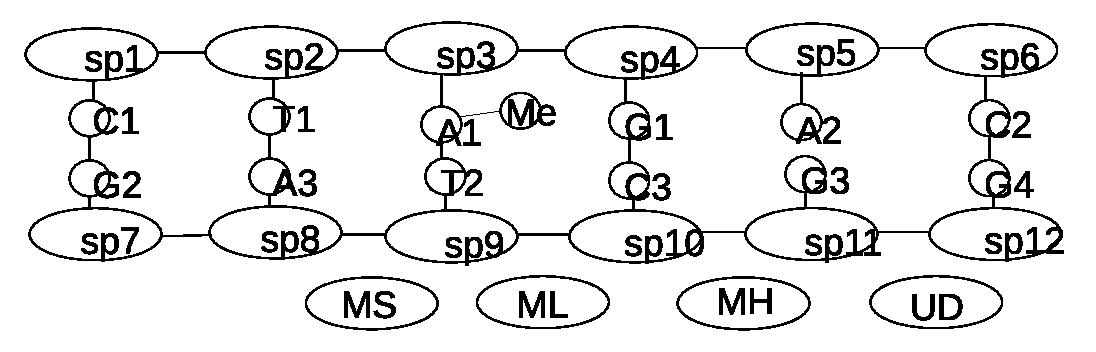
\includegraphics[width=1.0\textwidth]{mmr/state1}
  \caption[A six base pair DNA fragment.]{A six base pair DNA fragment, with a DNA mismatch and methylation of one strand. The proteins MutL, MutS, MutH, and UvrD are currently not bound to the DNA.}
  \label{fig:state1}
\end{figure}

We can model this similar to what we did before as:

$$\begin{array}{l}
(DP_1 \paral DP_2 \paral DP_3 \paral DP_4 \paral DP_5 \paral DP_6 \paral \\
C_1 \paral T_1 \paral A_1 \paral G_1 \paral A_2 \paral C_2 \paral \\
G_2 \paral A_3 \paral T_2 \paral C_3 \paral G_3 \paral G_4 \paral \\
DP_7 \paral DP_8 \paral DP_9 \paral DP_{10} \paral DP_{11} \paral DP_{12} \paral \\
Me \paral MutS \paral MutL \paral MutH \paral UvrD) \\
\setminus\{p3, p5, s, i, r, b, b, d, b, a, t, g, c, m, n, m2, l, o, s, u, v, w\} 
\end{array}$$ 

We leave out the restriction from now on for ease of reading. We number actions using subscripts where there is more than one instance, and set initial bonds as required. We get the following process:
%
\begin{flalign*}
&(p3_1,p5_1[1];s_1).DP_1' \paral (b_1[10],d_1).DP_1'' \paral (p3_2[1],p5_2[2];s_2).DP_2' \paral (b_2[8],d_2).DP_2'' \paral &&\\
&(p3_3[2],p5_3[3];s_3).DP_3' \paral (b_3[6],d_3).DP_3'' \paral (p3_4[3],p5_4[4];s_4).DP_4' \paral (b_4[9],d_4).DP_4'' \paral &&\\
&(p3_5[4],p5_5[5];s_5).DP_5' \paral (b_5[7],d_5).DP_5'' \paral (p3_6[5],p5_6;s_6).DP_6' \paral (b_6[11],d_6)).DP_6'' \paral  &&\\
&(b_1[6];i_1).(a_1[24],m_1[40];r_1).A_1' \paral (b_2[7];i_2).(a_2,m_2;r_2).A_2' \paral (b_3[18];i_3).(a_3[23],m_3;r_3).A_3' \paral &&\\
&(b_4[8];i_4).(t_1[23]:r_4).T_1' \paral (b_5[19];i_5).(t_2[24];r_5).T_2' \paral  (b_6[9];i_6).(g_1[25];r_6).G_1' \paral &&\\
&(b_7[17];i_7).(g_2[41];r_7).G_2' \paral (b_8[21];i_8).(g_3;r_8).G_3' \paral (b_9[22];i_9).(g_4[27];r_9).G_4' \paral&&\\
&(b_{10}[10];i_{10}).(c_1[41];r_{10}).C_1' \paral (b_{11}[11];i_{11}).(c_2[27];r_{11}).C_2' \paral (b_{12}[20];i_{12}).(c_3[25];r_{12}).C_3'  \paral&&\\
&(p3_7,p5_7[12];s_7).DP_7' \paral (b_7[17],d_7).DP_7'' \paral (p3_8[12],p5_8[13];s_8).DP_8' \paral (b_8[18],d_8).DP_8'' \paral &&\\
&(p3_9[13],p5_9[14];s_9).DP_9' \paral (b_9[19],d_9).DP_9'' \paral (p3_{10}[14],p5_{10}[15];s_{10}).DP_{10}' \paral (b_{10}[20],d_{10})).DP_{10}'' \paral  &&\\
&(p3_{11}[15],p5_{11}[16];s_{11}).DP_{11}' \paral (b_{11}[21],d_{11}).DP_{11'}' \paral (p3_{12}[16],p5_{12};s_{12}).DP_{12}' \paral (b_{12}[22],d_{12}).DP_{12}'' \paral  &&\\
&(m[40]).(n).Me'\paral (m2,m2).(l).MutS' \paral (l).(n).(o).MutL' \paral &&\\
&(o).(w).MutH' \paral (u;r).UvrD' \paral (v;s).UvrD''&&
\end{flalign*}

In this short DNA section , we firstly have a mismatch - $A_2$ and $G_3$ do not form an A/T or G/C pair as required. Secondly, methylation has happened on the old half of the strand, which means that an methyl group ($Me$) is attached to $A_1$. Note that there is no methyl group on $A_2$. This is because the methylation only happens on CTAG sequences. This happens via a specific protein, which we do not model, we just assume the end result. No $A$s would be methylated on the new half, even if they were in a CTAG sequence, since not enough time has passed for this to happen.

MutS can now bond to the $A$ and $G$ bases,  specifically to processes $A_2$ and $G_3$  via the $a_2$ and $g_3$ actions. This is the recognition of the mismatch. Not that the $a$ and $g$ actions are not available on matching pairs. So the bonding is not possible if the bases are properly paired, and also not if a Uracil is incorporated into the strand (as in the BER example). The transitions for creating the two bonds between $MutS$ and
$A_2$ and $G_3$ are as follows:

\begin{flalign*}
&\xrightarrow{m2a[28]} \xrightarrow{m2g[29]} (p3_1,p5_1[1];s_1).DP_1' \paral (b_1[10],d_1).DP_1'' \paral (p3_2[1],p5_2[2];s_2).DP_2' \paral &&\\
&(b_2[8],d_2).DP_2'' \paral (p3_3[2],p5_3[3];s_3).DP_3' \paral (b_3[6],d_3).DP_3'' (p3_4[3],p5_4[4];s_4).DP_4' \paral (b_4[9],d_4).DP_4'' \paral&&\\
&(p3_5[4],p5_5[5];s_5).DP_5' \paral (b_5[7],d_5).DP_5'' \paral (p3_6[5],p5_6;s_6).DP_6' \paral (b_6[11],d_6)).DP_6'' \paral  &&\\
&(b_1[6];i_1).(a_1[24],m_1[40];r_1).A_1' \paral (b_2[7];i_2).(\mathbf{a_2[28]},m_2;r_2).A_2' \paral (b_3[18];i_3).(a_3[23],m_3;r_3).A_3' \paral &&\\
&(b_4[8];i_4).(t_1[23]:r_4).T_1' \paral (b_5[19];i_5).(t_2[24];r_5).T_2' \paral  (b_6[9];i_6).(g_1[25];r_6).G_1' \paral &&\\
&(b_7[17];i_7).(g_2[41];r_7).G_2' \paral (b_8[21];i_8).(\mathbf{g_3[29]};r_8).G_3' \paral (b_9[22];i_9).(g_4[27];r_9).G_4' \paral&&\\
&(b_{10}[10];i_{10}).(c_1[41];r_{10}).C_1' \paral (b_{11}[11];i_{11}).(c_2[27];r_{11}).C_2' \paral (b_{12}[20];i_{12}).(c_3[25];r_{12}).C_3'  \paral&&\\
&(p3_7,p5_7[12];s_7).DP_7' \paral (b_7[17],d_7).DP_7'' \paral (p3_8[12],p5_8[13];s_8).DP_8' \paral (b_8[18],d_8).DP_8'' \paral &&\\
&(p3_9[13],p5_9[14];s_9).DP_9' \paral (b_9[19],d_9).DP_9'' \paral (p3_{10}[14],p5_{10}[15];s_{10}).DP_{10}' \paral (b_{10}[20],d_{10})).DP_{10}'' \paral &&\\
&(p3_{11}[15],p5_{11}[16];s_{11}).DP_{11}' \paral (b_{11}[21],d_{11}).DP_{11}'' \paral (p3_{12}[16],p5_{12};s_{12}).DP_{12}' \paral (b_{12}[22],d_{12}).DP_{12}'' \paral  &&\\
&(m[40]).(n).Me'\paral (\mathbf{m2[28],m2[29]}).(l).MutS' \paral (l).(n).(o).MutL' \paral &&\\
&(o).(w).MutH' \paral (u;r).UvrD' \paral (v;s).UvrD''&&
\end{flalign*}

Now it is possible for $MutL$ to bond to $MutS$ via a synchronisation on $l$ with key 30:

\begin{flalign*}
&\xrightarrow{ll[30]} (p3_1,p5_1[1];s_1).DP_1' \paral (b_1[10],d_1).DP_1'' \paral (p3_2[1],p5_2[2];s_2).DP_2' \paral (b_2[8],d_2).DP_2'' \paral &&\\
&(p3_3[2],p5_3[3];s_3).DP_3' \paral (b_3[6],d_3).DP_3'' \paral (p3_4[3],p5_4[4];s_4).DP_4' \paral (b_4[9],d_4).DP_4'' \paral &&\\
&(p3_5[4],p5_5[5];s_5).DP_5' \paral (b_5[7],d_5).DP_5'' \paral (p3_6[5],p5_6;s_6).DP_6' \paral (b_6[11],d_6)).DP_6'' \paral  &&\\
&(b_1[6];i_1).(a_1[24],m_1[40];r_1).A_1' \paral (b_2[7];i_2).(a_2[28],m_2;r_2).A_2' \paral (b_3[18];i_3).(a_3[23],m_3;r_3).A_3' \paral &&\\
&(b_4[8];i_4).(t_1[23]:r_4).T_1' \paral (b_5[19];i_5).(t_2[24];r_5).T_2' \paral  (b_6[9];i_6).(g_1[25];r_6).G_1' \paral &&\\
&(b_7[17];i_7).(g_2[41];r_7).G_2' \paral (b_8[21];i_8).(g_3[29];r_8).G_3' \paral (b_9[22];i_9).(g_4[27];r_9).G_4' \paral&&\\
&(b_{10}[10];i_{10}).(c_1[41];r_{10}).C_1' \paral (b_{11}[11];i_{11}).(c_2[27];r_{11}).C_2' \paral (b_{12}[20];i_{12}).(c_3[25];r_{12}).C_3'  \paral&&\\
&(p3_7,p5_7[12];s_7).DP_7' \paral (b_7[17],d_7).DP_7'' \paral (p3_8[12],p5_8[13];s_8).DP_8' \paral (b_8[18],d_8).DP_8'' \paral &&\\
&(p3_9[13],p5_9[14];s_9).DP_9' \paral (b_9[19],d_9).DP_9'' \paral (p3_{10}[14],p5_{10}[15];s_{10}).DP_{10}' \paral (b_{10}[20],d_{10})).DP_{10}'' \paral  &&\\
&(p3_{11}[15],p5_{11}[16];s_{11}).DP_{11}' \paral (b_{11}[21],d_{11}).DP_{11}'' \paral (p3_{12}[16],p5_{12};s_{12}).DP_{12}' \paral (b_{12}[22],d_{12}).DP_{12}'' \paral &&\\
&(m[40]).(n).Me'\paral (m2[28],m2[29]).(\mathbf{l[30]}).MutS' \paral (\mathbf{l[30]}).(n).(o).MutL' \paral &&\\
&(o).(w).MutH' \paral (u;r).UvrD' \paral (v;s).UvrD''&&
\end{flalign*}

$MutL$ now can bond with $Me$ via $n$, which means it detects which of the strands is methylated, and therefore the correct one:

\begin{flalign*}
&\xrightarrow{nn[31]} (p3_1,p5_1[1];s_1).DP_1' \paral (b_1[10],d_1).DP_1'' \paral (p3_2[1],p5_2[2];s_2).DP_2' \paral (b_2[8],d_2).DP_2'' \paral &&\\
&(p3_3[2],p5_3[3];s_3).DP_3' \paral (b_3[6],d_3).DP_3'' \paral (p3_4[3],p5_4[4];s_4).DP_4' \paral (b_4[9],d_4).DP_4'' \paral &&\\
&(p3_5[4],p5_5[5];s_5).DP_5' \paral (b_5[7],d_5).DP_5'' \paral (p3_6[5],p5_6;s_6).DP_6' \paral (b_6[11],d_6)).DP_6'' \paral  &&\\
&(b_1[6];i_1).(a_1[24],m_1[40];r_1).A_1' \paral (b_2[7];i_2).(a_2[28],m_2;r_2).A_2' \paral (b_3[18];i_3).(a_3[23],m_3;r_3).A_3' \paral &&\\
&(b_4[8];i_4).(t_1[23]:r_4).T_1' \paral (b_5[19];i_5).(t_2[24];r_5).T_2' \paral  (b_6[9];i_6).(g_1[25];r_6).G_1' \paral &&\\
&(b_7[17];i_7).(g_2[41];r_7).G_2' \paral (b_8[21];i_8).(g_2[29];r_8).G_3' \paral (b_9[22];i_9).(g_2[27];r_9).G_4' \paral&&\\
&(b_9[10];i_9).(c_1[41];r_{10}).C_1' \paral (b_{10}[11];i_{10}).(c_2[27];r_{11}).C_2' \paral (b_{11}[20];i_{11}).(c_3[25];r_{12}).C_3'  \paral&&\\
&(p3_7,p5_7[12];s_7).DP_7' \paral (b_7[17],d_7).DP_7'' \paral (p3_8[12],p5_8[13];s_8).DP_8' \paral (b_8[18],d_8).DP_8'' \paral &&\\
&(p3_9[13],p5_9[14];s_9).DP_9' \paral (b_9[19],d_9).DP_9'' \paral (p3_{10}[14],p5_{10}[15];s_{10}).DP_{10}' \paral (b_{10}[20],d_{10})).DP_{10}'' \paral &&\\
&(p3_{11}[15],p5_{11}[16];s_{11}).DP_{11}' \paral (b_{11}[21],d_{11}).DP_{11}'' \paral (p3_{12}[16],p5_{12};s_{12}).DP_{12}' \paral (b_{12}[22],d_{12}).DP_{12}'' \paral  &&\\
&S(m[40]).(\mathbf{n[31]}).Me'\paral (m2[28],m2[29]).(l[30]).MutS' \paral (l[30]).(\mathbf{n[31]}).(o).MutL' \paral &&\\
&(o).(w).MutH' \paral (u;r).UvrD' \paral (v;s).UvrD''&&
\end{flalign*}

MutL is now ready to recruit MutH:

\begin{flalign*}
&\xrightarrow{oo[32]} (p3_1,p5_1[1];s_1).DP_1' \paral (b_1[10],d_1).DP_1'' \paral (p3_2[1],p5_2[2];s_2).DP_2' \paral (b_2[8],d_2).DP_2'' \paral&&\\ 
&(p3_3[2],p5_3[3];s_3).DP_3' \paral (b_3[6],d_3).DP_3'' \paral (p3_4[3],p5_4[4];s_4).DP_4' \paral (b_4[9],d_4).DP_4'' \paral &&\\
&(p3_5[4],p5_5[5];s_5).DP_5' \paral (b_5[7],d_5).DP_5'' \paral (p3_6[5],p5_6;s_6).DP_6' \paral (b_6[11],d_6)).DP_6'' \paral  &&\\
&(b_1[6];i_1).(a_1[24],m_1[40];r_1).A_1' \paral (b_2[7];i_2).(a_2[28],m_2;r_2).A_2' \paral (b_3[18];i_3).(a_3[23],m_3;r_3).A_3' \paral &&\\
&(b_4[8];i_4).(t_1[23]:r_4).T_1' \paral (b_5[19];i_5).(t_2[24];r_5).T_2' \paral  (b_6[9];i_6).(g_1[25];r_6).G_1' \paral &&\\
&(b_7[17];i_7).(g_2[41];r_7).G_2' \paral (b_8[21];i_8).(g_3[29];r_8).G_3' \paral (b_9[22];i_9).(g_4[27];r_9).G_4' \paral&&\\
&(b_{10}[10];i_{10}).(c_1[41];r_{10}).C_1' \paral (b_{11}[11];i_{11}).(c_2[27];r_{11}).C_2' \paral (b_{12}[20];i_{12}).(c_3[25];r_{12}).C_3'  \paral&&\\
&(p3_7,p5_7[12];s_7).DP_7' \paral (b_7[17],d_7).DP_7'' \paral (p3_8[12],p5_8[13];s_8).DP_8' \paral (b_8[18],d_8).DP_8'' \paral &&\\
&(p3_9[13],p5_9[14];s_9).DP_9' \paral (b_9[19],d_9).DP_9'' \paral (p3_{10}[14],p5_{10}[15];s_{10}).DP_{10}' \paral (b_{10}[20],d_{10})).DP_{10}'' \paral &&\\
& (p3_{11}[15],p5_{11}[16];s_{11}).DP_{11}' \paral (b_{11}[21],d_{11}).DP_{11}'' \paral (p3_{12}[16],p5_{12};s_{12}).DP_{12}' \paral (b_{12}[22],d_{12}).DP_{12}'' \paral &&\\
&(m[40]).(n[31]).Me'\paral (m2[28],m2[29]).(l[30]).MutS' \paral (l[30]).(n[31]).(\mathbf{o[32]}).MutL' \paral &&\\
&(\mathbf{o[32]}).(w).MutH' \paral (u;r).UvrD' \paral (v;s).UvrD''&&
\end{flalign*}

MutH is now ready to cleave the DNA at the right location:

\begin{flalign*}
&\xrightarrow{\{ws[33],\underline{p}[13]\}} (p3_1,p5_1[1];s_1).DP_1' \paral (b_1[10],d_1).DP_1'' \paral (p3_2[1],p5_2[2];s_2).DP_2' \paral &&\\
&(b_2[8],d_2).DP_2'' \paral (p3_3[2],p5_3[3];s_3).DP_3' \paral (b_3[6],d_3).DP_3'' \paral (p3_4[3],p5_4[4];s_4).DP_4' \paral (b_4[9],d_4).DP_4'' \paral &&\\
&(p3_5[4],p5_5[5];s_5).DP_5' \paral (b_5[7],d_5).DP_5'' \paral (p3_6[5],p5_6;s_6).DP_6' \paral (b_6[11],d_6)).DP_6'' \paral  &&\\
&(b_1[6];i_1).(a_1[24],m_1[40];r_1).A_1' \paral (b_2[7];i_2).(a_2[28],m_2;r_2).A_2' \paral (b_3[18];i_3).(a_3[23],m_3;r_3).A_3' \paral &&\\
&(b_4[8];i_4).(t_1[23]:r_4).T_1' \paral (b_5[19];i_5).(t_2[24];r_5).T_2' \paral  (b_6[9];i_6).(g_1[25];r_6).G_1' \paral &&\\
&(b_7[17];i_7).(g_2[41];r_7).G_2' \paral (b_8[21];i_8).(g_3[29];r_8).G_3' \paral (b_9[22];i_9).(g_4[27];r_9).G_4' \paral&&\\
&(b_{10}[10];i_{10}).(c_1[41];r_{10}).C_1' \paral (b_{11}[11];i_{11}).(c_2[27];r_{11}).C_2' \paral (b_{12}[20];i_{12}).(c_3[25];r_{12}).C_3'  \paral&&\\
&(p3_7,p5_7[12];s_7).DP_7' \paral (b_7[17],d_7).DP_7'' \paral (p3_8[12],\mathbf{p5_8};s_8).DP_8' \paral (b_8[18],d_8).DP_8'' \paral &&\\
&(\mathbf{p3_9},p5_9[14];\mathbf{s_9[33]}).DP_9' \paral (b_9[19],d_9).DP_9'' \paral (p3_{10}[14],p5_{10}[15];s_{10}).DP_{10}' \paral (b_{10}[20],d_{10})).DP_{10}'' \paral  &&\\
&(p3_{11}[15],p5_{11}[16];s_{11}).DP_{11}' \paral (b_{11}[21],d_{11}).DP_{11}'' \paral (p3_{12}[16],p5_{12};s_{12}).DP_{12}' \paral (b_{12}[22],d_{12}).DP_{12}'' \paral  &&\\
&(m[40]).(n[31]).Me'\paral (m2[28],m2[29]).(l[30]).MutS' \paral (l[30]).(n[31]).(o[32]).MutL' \paral &&\\
&(o[32]).(\mathbf{w[33]}).MutH' \paral (u;r).UvrD' \paral (v;s).UvrD''&&
\end{flalign*}

Next, {\em promotion} happens, which moves the bond with key 33 from weak action $s_9$ to strong action $p3_9$:

\begin{flalign*}
&\overset{ \rulename{prom}}\Rightarrow (p3_1,p5_1[1];s_1).DP_1' \paral (b_1[10],d_1).DP_1'' \paral (p3_2[1],p5_2[2];s_2).DP_2' \paral &&\\
&(b_2[8],d_2).DP_2'' \paral (p3_3[2],p5_3[3];s_3).DP_3' \paral (b_3[6],d_3).DP_3'' \paral (p3_4[3],p5_4[4];s_4).DP_4' \paral (b_4[9],d_4).DP_4'' \paral &&\\
&(p3_5[4],p5_5[5];s_5).DP_5' \paral (b_5[7],d_5).DP_5'' \paral (p3_6[5],p5_6;s_6).DP_6' \paral (b_6[11],d_6)).DP_6'' \paral  &&\\
&(b_1[6];i_1).(a_1[24],m_1[40];r_1).A_1' \paral (b_2[7];i_2).(a_2[28],m_2;r_2).A_2' \paral (b_3[18];i_3).(a_3[23],m_3;r_3).A_3' \paral &&\\
&(b_4[8];i_4).(t_1[23]:r_4).T_1' \paral (b_5[19];i_5).(t_2[24];r_5).T_2' \paral  (b_6[9];i_6).(g_1[25];r_6).G_1' \paral &&\\
&(b_7[17];i_7).(g_2[41];r_7).G_2' \paral (b_8[21];i_8).(g_3[29];r_8).G_3' \paral (b_9[22];i_9).(g_4[27];r_9).G_4' \paral&&\\
&(b_{10}[10];i_{10}).(c_1[41];r_{10}).C_1' \paral (b_{11}[11];i_{11}).(c_2[27];r_{11}).C_2' \paral (b_{12}[20];i_{12}).(c_3[25];r_{10}).C_3'  \paral&&\\
&(p3_7,p5_7[12];s_7).DP_7' \paral (b_7[17],d_7).DP_7'' \paral (p3_8[12],p5_8;s_8).DP_8' \paral (b_8[18],d_8).DP_8'' \paral &&\\
&(\mathbf{p3_9[33]},p5_9[14];\mathbf{s_9}).DP_9' \paral (b_9[19],d_9).DP_9'' \paral (p3_{10}[14],p5_{10}[15];s_{10}).DP_{10}' \paral (b_{10}[20],d_{10})).DP_{10}'' \paral  &&\\
&(p3_{11}[15],p5_{11}[16];s_{11}).DP_{11}' \paral (b_{11}[21],d_{11}).DP_{11}'' \paral (p3_{12}[16],p5_{12};s_{12}).DP_{12}' \paral (b_{12}[22],d_{12}).DP_{12}'' \paral  &&\\
&(m[40]).(n[31]).Me'\paral (m2[28],m2[29]).(l[30]).MutS' \paral (l[30]).(n[31]).(o[32]).MutL' \paral &&\\
&(o[32]).(\mathbf{w[33]}).MutH' \paral (u;r).UvrD' \paral (v;s).UvrD''&&
\end{flalign*}

Note that execution of $s_9$ on $DP_9$ leads to breaking a bond between two deoxyribose/phosphate groups. Specifically, bond 33 from $MutH$ to $DP_9$ via actions $w$ and $s$ is formed and bond 13 between $p5$ in $DP_8$ and $p3$ in  $DP_9$ is broken. We use a concerted action and rewriting for this. The situation after this step is shown in Figure~\ref{fig:state2}. This has now the right DNA strand cleaved.

\begin{figure}[h!]
\psfrag{dp1}{${\mathrm{DP_1}}$}
\psfrag{dp2}{${\mathrm{DP_2}}$}
\psfrag{dp3}{${\mathrm{DP_3}}$}
\psfrag{dp4}{${\mathrm{DP_4}}$}
\psfrag{dp5}{${\mathrm{DP_5}}$}
\psfrag{dp6}{${\mathrm{DP_6}}$}
\psfrag{dp7}{${\mathrm{DP_7}}$}
\psfrag{dp8}{${\mathrm{DP_8}}$}
\psfrag{dp9}{${\mathrm{DP_9}}$}
\psfrag{dp10}{${\mathrm{DP_{10}}}$}
\psfrag{dp11}{${\mathrm{DP_{11}}}$}
\psfrag{dp12}{${\mathrm{DP_{12}}}$}
\psfrag{A1}{${\mathrm{A_1}}$}
\psfrag{A2}{${\mathrm{A_2}}$}
\psfrag{A3}{${\mathrm{A_3}}$}
\psfrag{T1}{${\mathrm{T_1}}$}
\psfrag{T2}{${\mathrm{T_2}}$}
\psfrag{C1}{${\mathrm{C_1}}$}
\psfrag{C2}{${\mathrm{C_2}}$}
\psfrag{C3}{${\mathrm{C_3}}$}
\psfrag{G1}{${\mathrm{G_1}}$}
\psfrag{G2}{${\mathrm{G_2}}$}
\psfrag{G3}{${\mathrm{G_3}}$}
\psfrag{G4}{${\mathrm{G_4}}$}
\psfrag{Me}{${\mathrm{Me}}$}
\psfrag{MS}{${\mathrm{MutS}}$}
\psfrag{ML}{${\mathrm{MutL}}$}
\psfrag{MH}{${\mathrm{MutH}}$}
\psfrag{UD}{${\mathrm{UvrD}}$}
  \centering
    \includegraphics[width=1.0\textwidth]{mmr/state2}
  \caption[A six base pair DNA fragment.]{A six base pair DNA fragment, with a DNA mismatch and methylation of one strand. The mismatch has been detected by MutS and MutH and MutL have been recruited. MutL has detected the methylation, and MutH has cleaved the strand containing the wrong base.}
  \label{fig:state2}
\end{figure}

Now the UvrD protein can use the cleavage to remove pairs of deoxyribose/phosphate groups and bases. This works as follows:

\begin{flalign*}
&\xrightarrow{\{sv[34],\underline{at}[14]\}}  \overset{ \rulename{prom}}\Rightarrow \xrightarrow{\{ur[35],\underline{at}[24]\}}  \overset{ \rulename{prom}}\Rightarrow (p3_1,p5_1[1];s_1).DP_1' \paral (b_1[10],d_1).DP_1'' \paral (p3_2[1],p5_2[2];s_2).DP_2' \paral &&\\
&(b_2[8],d_2).DP_2'' \paral (p3_3[2],p5_3[3];s_3).DP_3' \paral (b_3[6],d_3).DP_3'' \paral (p3_4[3],p5_4[4];s_4).DP_4' \paral (b_4[9],d_4).DP_4'' \paral &&\\
&(p3_5[4],p5_5[5];s_5).DP_5' \paral (b_5[7],d_5).DP_5'' \paral (p3_6[5],p5_6;s_6).DP_6' \paral (b_6[11],d_6)).DP_6'' \paral  &&\\
&(b_1[6];i_1).(\mathbf{a_1},m_1[40];r_1).A_1' \paral (b_2[7];i_2).(a_2[28],m_2;r_2).A_2' \paral (b_3[18];i_3).(a_3[23],m_3;r_3).A_3' \paral &&\\
&(b_4[8];i_4).(t_1[23]:r_4).T_1' \paral (b_5[19];i_5).(\mathbf{t_2[35]};r_5).T_2' \paral  (b_6[9];i_6).(g_1[25];r_6).G_1' \paral &&\\
&(b_7[17];i_7).(g_2[41];r_7).G_2' \paral (b_8[21];i_8).(g_3[29];r_8).G_3' \paral (b_9[22];i_9).(g_4[27];r_9).G_4' \paral&&\\
&(b_{10}[10];i_{10}).(c_1[41];r_{10}).C_1' \paral (b_{11}[11];i_{11}).(c_2[27];r_{11}).C_2' \paral (b_{12}[20];i_{12}).(c_3[25];r_{12}).C_3'  \paral&&\\
&(p3_7,p5_7[12];s_7).DP_7' \paral (b_7[17],d_7).DP_7'' \paral (p3_8[12],p5_8;s_8).DP_8' \paral (b_8[18],d_8).DP_8'' &&\\
&\paral (p3_9[33],p5_9;s_9).DP_9' \paral (b_9[19],d_9).DP_9'' \paral (\mathbf{p3_{10}[34]},p5_{10}[15];s_{10}).DP_{10}' \paral (b_{10}[20],d_{10})).DP_{10}'' \paral  &&\\
&(p3_{11}[15],p5_{11}[16];s_{11}).DP_{11}' \paral (b_{11}[21],d_{11}).DP_{11}'' \paral (p3_{12}[16],p5_{12};s_{12}).DP_{12}' \paral (b_{12}[22],d_{12}).DP_{12}'' \paral  &&\\
&(m[40]).(n[31]).Me'\paral (m2[28],m2[29]).(l[30]).MutS' \paral (l[30]).(n[31]).(o[32]).MutL' \paral &&\\
&(o[32]).(w[33]).MutH' \paral (\mathbf{u[35]};r).UvrD' \paral (\mathbf{v[34]};s).UvrD''&&
\end{flalign*}

$UD$ is attached not to $DP_9$ initially here, but to $DP_10$. If it would be attached to $DP_9$, it would have no connection to the DNA strand anymore once the bonds of $DP_9$ and $T_2$ to the DNA strand are broken.

The removal of the first base and deoxyribose/phosphate group is shown in Figure~\ref{fig:state3}. The dashed lines indicate the bonds being broken and formed during concerted actions. The two concerted actions are shown by thin (34/14) and bold dashed lines (35/24).

\begin{figure}[h!]
\psfrag{dp1}{${\mathrm{DP_1}}$}
\psfrag{dp2}{${\mathrm{DP_2}}$}
\psfrag{dp3}{${\mathrm{DP_3}}$}
\psfrag{dp4}{${\mathrm{DP_4}}$}
\psfrag{dp5}{${\mathrm{DP_5}}$}
\psfrag{dp6}{${\mathrm{DP_6}}$}
\psfrag{dp7}{${\mathrm{DP_7}}$}
\psfrag{dp8}{${\mathrm{DP_8}}$}
\psfrag{dp9}{${\mathrm{DP_9}}$}
\psfrag{dp10}{${\mathrm{DP_{10}}}$}
\psfrag{dp11}{${\mathrm{DP_{11}}}$}
\psfrag{dp12}{${\mathrm{DP_{12}}}$}
\psfrag{A1}{${\mathrm{A_1}}$}
\psfrag{A2}{${\mathrm{A_2}}$}
\psfrag{A3}{${\mathrm{A_3}}$}
\psfrag{T1}{${\mathrm{T_1}}$}
\psfrag{T2}{${\mathrm{T_2}}$}
\psfrag{C1}{${\mathrm{C_1}}$}
\psfrag{C2}{${\mathrm{C_2}}$}
\psfrag{C3}{${\mathrm{C_3}}$}
\psfrag{G1}{${\mathrm{G_1}}$}
\psfrag{G2}{${\mathrm{G_2}}$}
\psfrag{G3}{${\mathrm{G_3}}$}
\psfrag{G4}{${\mathrm{G_4}}$}
\psfrag{Me}{${\mathrm{Me}}$}
\psfrag{MS}{${\mathrm{MutS}}$}
\psfrag{ML}{${\mathrm{MutL}}$}
\psfrag{MH}{${\mathrm{MutH}}$}
\psfrag{UD}{${\mathrm{UvrD}}$}
  \centering
    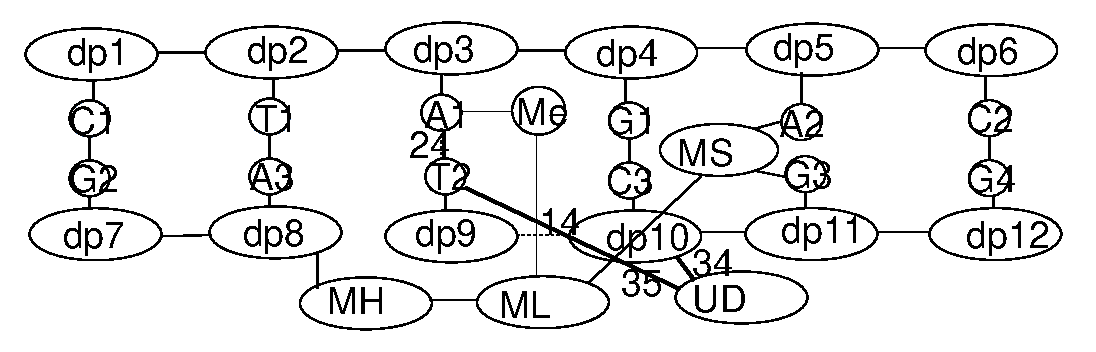
\includegraphics[width=1.0\textwidth]{mmr/state3}
  \caption[A six base pair DNA fragment.]{A six base pair DNA fragment, with a DNA mismatch and methylation of one strand. UvrD has now bonded to $T_2$ and $DP_{10}$, breaking the bonds of those molecules to the rest of the DNA via concerted actions (shown as dotted lines). In a next step, UvrD can now ``walk'' along the DNA strand, and remove the next pair.}
  \label{fig:state3}
\end{figure}

From here, UvrD can ``walk'' along the strand. As opposed to BER, the bonds between the base pairs are now broken during the walk. In parallel, the bonds between the deoxyribose/phosphate groups are also broken as UvrD progresses. We write this as two separate concerted transitions here for clarity:

\begin{flalign*}
&\xrightarrow{\{ss[36],\underline{vp3}[34],\underline{p}[15]\}} \overset{ \rulename{prom}}\Rightarrow  &&\\
& (p3_1,p5_1[1];s_1).DP_1' \paral (b_1[10],d_1).DP_1'' \paral (p3_2[1],p5_2[2];s_2).DP_2' \paral 
(b_2[8],d_2).DP_2'' \paral && \\
& (p3_3[2],p5_3[3];s_3).DP_3' \paral (b_3[6],d_3).DP_3'' \paral (p3_4[3],p5_4[4];s_4).DP_4' \paral (b_4[9],d_4).DP_4'' \paral &&\\
&(p3_5[4],p5_5[5];s_5).DP_5' \paral (b_5[7],d_5).DP_5'' \paral (p3_6[5],p5_6;s_6).DP_6' \paral (b_6[11],d_6)).DP_6'' \paral  &&\\
&(b_1[6];i_1).(a_1,m_1[40];r).A_1' \paral (b_2[7];i_2).(a_2[28],m_2;r).A_2' \paral (b_3[18];i_3).(a_3[23],m_3;r).A_3' \paral &&\\
&(b_4[8];i_4).(t_1[23]:r_1).T_1' \paral (b_5[19];i_5).(t_2[35];r_2).T_2' \paral  (b_6[9];i_6).(g_1[25];r_3).G_1' \paral &&\\
&(b_7[17];i_7).(g_2[41];r_4).G_2' \paral (b_8[21];i_8).(g_2[29];r_4).G_3' \paral (b_9[22];i_9).(g_3[27];r_5).G_4' \paral&&\\
&(b_9[10];i_9).(c_1[41];r_6).C_1' \paral (b_{10}[11];i_{10}).(c_2[27];r_7).C_2' \paral (b_{11}[20];i_{11}).(c_3[25];r_8).C_3'  \paral&&\\
&(p3_7,p5_7[12];s_7).DP_7' \paral (b_7[17],d_7).DP_7'' \paral (p3_8[12],p5_8;s_8).DP_8' \paral (b_8[18],d_8).DP_8'' \paral &&\\
&(p3_9[33],p5_9;s_9).DP_9' \paral (b_9[19],d_9).DP_9'' \paral (\mathbf{p3_{10},p5_{10}};s_{10}).DP_{10}' \paral (b_{10}[20],d_{10})).DP_{10}'' \paral &&\\
&(\mathbf{p3_{11}[36]},p5_{11}[16];s_{11}).DP_{11}' \paral (b_{11}[21],d_{11}).DP_{11}'' \paral (p3_{12}[16],p5_{12};s_{12}).DP_{12}' \paral (b_{12}[22],d_{12}).DP_{12}'' \paral  &&\\
&(m[40]).(n[31]).Me'\paral (m2[28],m2[29]).(l[30]).MutS' \paral (l[30]).(n[31]).(o[32]).MutL' \paral &&\\
&(o[32]).(w[33]).MutH' \paral (u[35];r).UvrD' \paral (\mathbf{v[36]};s).UvrD''&&
\end{flalign*}

\begin{flalign*}
&\xrightarrow{\{rr[37],\underline{tu}[35],\underline{cg}[25]\}} \overset{ \rulename{prom}}\Rightarrow  &&\\
& (p3_1,p5_1[1];s_1).DP_1' \paral (b_1[10],d_1).DP_1'' \paral (p3_2[1],p5_2[2];s_2).DP_2' \paral 
(b_2[8],d_2).DP_2'' \paral && \\
& (p3_3[2],p5_3[3];s_3).DP_3' \paral (b_3[6],d_3).DP_3'' \paral (p3_4[3],p5_4[4];s_4).DP_4' \paral (b_4[9],d_4).DP_4'' \paral &&\\
&(p3_5[4],p5_5[5];s_5).DP_5' \paral (b_5[7],d_5).DP_5'' \paral (p3_6[5],p5_6;s_6).DP_6' \paral (b_6[11],d_6)).DP_6'' \paral  &&\\
&(b_1[6];i_1).(a_1,m_1[40];r).A_1' \paral (b_2[7];i_2).(a_2[28],m_2;r).A_2' \paral (b_3[18];i_3).(a_3[23],m_3;r).A_3' \paral &&\\
&(b_4[8];i_4).(t_1[23]:r_1).T_1' \paral (b_5[19];i_5).(\mathbf{t_2};r_2).T_2' \paral  (b_6[9];i_6).(\mathbf{g_1};r_3).G_1' \paral &&\\
&(b_7[17];i_7).(g_2[41];r_4).G_2' \paral (b_8[21];i_8).(g_2[29];r_4).G_3' \paral (b_9[22];i_9).(g_3[27];r_5).G_4' \paral&&\\
&(b_9[10];i_9).(c_1[41];r_6).C_1' \paral (b_{10}[11];i_{10}).(c_2[27];r_7).C_2' \paral (b_{11}[20];i_{11}).(\mathbf{c_3[37]};r_8).C_3'  \paral&&\\
&(p3_7,p5_7[12];s_7).DP_7' \paral (b_7[17],d_7).DP_7'' \paral (p3_8[12],p5_8;s_8).DP_8' \paral (b_8[18],d_8).DP_8'' \paral &&\\
&(p3_9[33],p5_9;s_9).DP_9' \paral (b_9[19],d_9).DP_9'' \paral (p3_{10},p5_{10};s_{10}).DP_{10}' \paral (b_{10}[20],d_{10})).DP_{10}'' \paral &&\\
&(p3_{11}[36],p5_{11}[16];s_{11}).DP_{11}' \paral (b_{11}[21],d_{11}).DP_{11}'' \paral (p3_{12}[16],p5_{12};s_{12}).DP_{12}' \paral (b_{12}[22],d_{12}).DP_{12}'' \paral  &&\\
&(m[40]).(n[31]).Me'\paral (m2[28],m2[29]).(l[30]).MutS' \paral (l[30]).(n[31]).(o[32]).MutL' \paral &&\\
&(o[32]).(w[33]).MutH' \paral (\mathbf{u[37]};r).UvrD' \paral (v[36];s).UvrD''&&
\end{flalign*}






This is shown in Figure~\ref{fig:state4}. Here, the first  base and deoxyribose/phosphate group has been removed (no longer shown in Figure~\ref{fig:state4}) and UvrD is moving to the next  base and deoxyribose/phosphate group, again removing them. The two concerted actions are shown by thin (36/15) and bold dashed lines (37/25).
\textbf{Problem: The three actions concerted action is not part of the calculus so far.}

\begin{figure}[h!]
\psfrag{dp1}{${\mathrm{DP_1}}$}
\psfrag{dp2}{${\mathrm{DP_2}}$}
\psfrag{dp3}{${\mathrm{DP_3}}$}
\psfrag{dp4}{${\mathrm{DP_4}}$}
\psfrag{dp5}{${\mathrm{DP_5}}$}
\psfrag{dp6}{${\mathrm{DP_6}}$}
\psfrag{dp7}{${\mathrm{DP_7}}$}
\psfrag{dp8}{${\mathrm{DP_8}}$}
\psfrag{dp9}{${\mathrm{DP_9}}$}
\psfrag{dp10}{${\mathrm{DP_{10}}}$}
\psfrag{dp11}{${\mathrm{DP_{11}}}$}
\psfrag{dp12}{${\mathrm{DP_{12}}}$}
\psfrag{A1}{${\mathrm{A_1}}$}
\psfrag{A2}{${\mathrm{A_2}}$}
\psfrag{A3}{${\mathrm{A_3}}$}
\psfrag{T1}{${\mathrm{T_1}}$}
\psfrag{T2}{${\mathrm{T_2}}$}
\psfrag{C1}{${\mathrm{C_1}}$}
\psfrag{C2}{${\mathrm{C_2}}$}
\psfrag{C3}{${\mathrm{C_3}}$}
\psfrag{G1}{${\mathrm{G_1}}$}
\psfrag{G2}{${\mathrm{G_2}}$}
\psfrag{G3}{${\mathrm{G_3}}$}
\psfrag{G4}{${\mathrm{G_4}}$}
\psfrag{Me}{${\mathrm{Me}}$}
\psfrag{MS}{${\mathrm{MutS}}$}
\psfrag{ML}{${\mathrm{MutL}}$}
\psfrag{MH}{${\mathrm{MutH}}$}
\psfrag{UD}{${\mathrm{UvrD}}$}
  \centering
    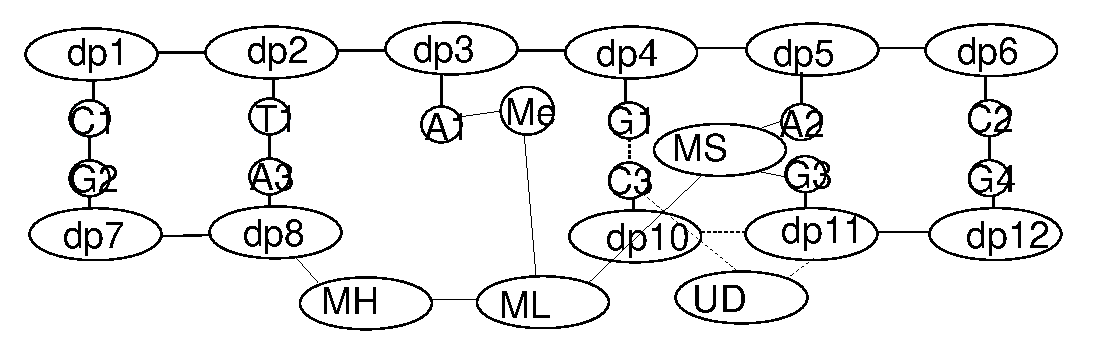
\includegraphics[width=1.0\textwidth]{mmr/state4}
  \caption[A six base pair DNA fragment.]{A six base pair DNA fragment, with a DNA mismatch and methylation of one strand. UvrD has now bonded to $C_2$ and $DP_{10}$, breaking the bonds of those molecules to the rest of the DNA via concerted actions (shown as dotted lines). This process can conitine for more pairs.}
  \label{fig:state4}
\end{figure}

This process can continue until the offending base has been removed. Figure~\ref{fig:state6} shows the removal of the offending base. We do not model how the number of base pairs to remove is determined. In reality, that number is not fixed, but is determined by the interal workings of the protein, where the number is statistically distributed. Once this is done and the MutH, MutL, and MutS proteins have detached we get the situation shown in Figure~\ref{fig:state7}. This is now ready for other proteins to replace the bases and and deoxyribose/phosphate groups. Notice that the remaining strand contains the necessary information for this, in particular only a T base can be put in opposite the A base. Note that the methyl group stays attached to $A_1$, since it is still an old DNA strand. Also the appropriate groups in the new, lower half will be methylated, so that both strands are marked as old material after the next DNA duplication process.

The modelling done so far does not involve any spatial configurataions. As in the BER example, this means that UvrD could bond to any deoxyribose/phosphate group, not just the neighbouring one. It also means that we have not modelled the formation of the loop in the DNA, which is crucial for cleaving the correct strand.

\begin{figure}[h!]
\psfrag{dp1}{${\mathrm{DP_1}}$}
\psfrag{dp2}{${\mathrm{DP_2}}$}
\psfrag{dp3}{${\mathrm{DP_3}}$}
\psfrag{dp4}{${\mathrm{DP_4}}$}
\psfrag{dp5}{${\mathrm{DP_5}}$}
\psfrag{dp6}{${\mathrm{DP_6}}$}
\psfrag{dp7}{${\mathrm{DP_7}}$}
\psfrag{dp8}{${\mathrm{DP_8}}$}
\psfrag{dp9}{${\mathrm{DP_9}}$}
\psfrag{dp10}{${\mathrm{DP_{10}}}$}
\psfrag{dp11}{${\mathrm{DP_{11}}}$}
\psfrag{dp12}{${\mathrm{DP_{12}}}$}
\psfrag{A1}{${\mathrm{A_1}}$}
\psfrag{A2}{${\mathrm{A_2}}$}
\psfrag{A3}{${\mathrm{A_3}}$}
\psfrag{T1}{${\mathrm{T_1}}$}
\psfrag{T2}{${\mathrm{T_2}}$}
\psfrag{C1}{${\mathrm{C_1}}$}
\psfrag{C2}{${\mathrm{C_2}}$}
\psfrag{C3}{${\mathrm{C_3}}$}
\psfrag{G1}{${\mathrm{G_1}}$}
\psfrag{G2}{${\mathrm{G_2}}$}
\psfrag{G3}{${\mathrm{G_3}}$}
\psfrag{G4}{${\mathrm{G_4}}$}
\psfrag{Me}{${\mathrm{Me}}$}
\psfrag{MS}{${\mathrm{MutS}}$}
\psfrag{ML}{${\mathrm{MutL}}$}
\psfrag{MH}{${\mathrm{MutH}}$}
\psfrag{UD}{${\mathrm{UvrD}}$}
  \centering
    \includegraphics[width=1.0\textwidth]{mmr/state6}
  \caption[A six base pair DNA fragment.]{A six base pair DNA fragment, with a DNA mismatch and methylation of one strand. UvrD has now bonded to $G_3$ (the offendingn base) and $DP_{11}$, breaking the bonds of those molecules to the rest of the DNA via concerted actions (shown as dotted lines). The offending base is removed after this step.}
  \label{fig:state6}
\end{figure}

\begin{figure}[h!]
\psfrag{dp1}{${\mathrm{DP_1}}$}
\psfrag{dp2}{${\mathrm{DP_2}}$}
\psfrag{dp3}{${\mathrm{DP_3}}$}
\psfrag{dp4}{${\mathrm{DP_4}}$}
\psfrag{dp5}{${\mathrm{DP_5}}$}
\psfrag{dp6}{${\mathrm{DP_6}}$}
\psfrag{dp7}{${\mathrm{DP_7}}$}
\psfrag{dp8}{${\mathrm{DP_8}}$}
\psfrag{dp9}{${\mathrm{DP_9}}$}
\psfrag{dp10}{${\mathrm{DP_{10}}}$}
\psfrag{dp11}{${\mathrm{DP_{11}}}$}
\psfrag{dp12}{${\mathrm{DP_{12}}}$}
\psfrag{A1}{${\mathrm{A_1}}$}
\psfrag{A2}{${\mathrm{A_2}}$}
\psfrag{A3}{${\mathrm{A_3}}$}
\psfrag{T1}{${\mathrm{T_1}}$}
\psfrag{T2}{${\mathrm{T_2}}$}
\psfrag{C1}{${\mathrm{C_1}}$}
\psfrag{C2}{${\mathrm{C_2}}$}
\psfrag{C3}{${\mathrm{C_3}}$}
\psfrag{G1}{${\mathrm{G_1}}$}
\psfrag{G2}{${\mathrm{G_2}}$}
\psfrag{G3}{${\mathrm{G_3}}$}
\psfrag{G4}{${\mathrm{G_4}}$}
\psfrag{Me}{${\mathrm{Me}}$}
\psfrag{MS}{${\mathrm{MutS}}$}
\psfrag{ML}{${\mathrm{MutL}}$}
\psfrag{MH}{${\mathrm{MutH}}$}
\psfrag{UD}{${\mathrm{UvrD}}$}
  \centering
    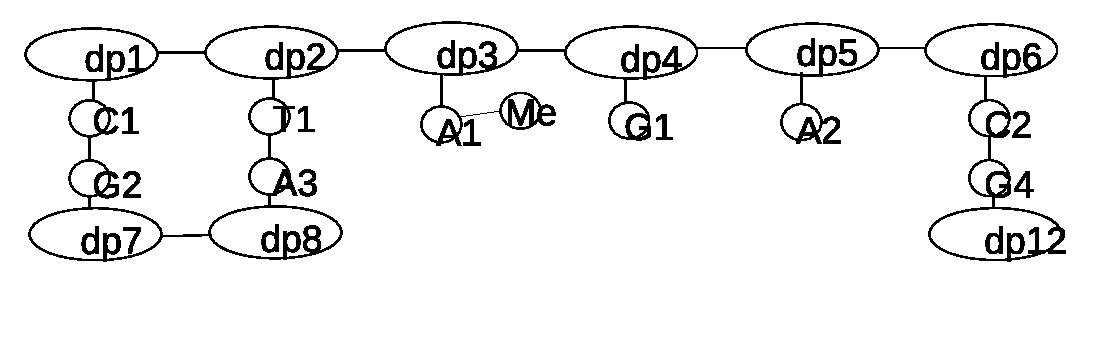
\includegraphics[width=1.0\textwidth]{mmr/state7}
  \caption[A six base pair DNA fragment.]{A six base pair DNA fragment, with a gap in one strand produced by MMR. This is now ready to replaced with correct information.}
  \label{fig:state7}
\end{figure}



%
\section{Conclusion}

In this paper, we have used a Calculus of Covalent Bonding  to model an important gene repair pathway, namely the DNA Mismatch Repair (MMR) mechanism. Since the molecules that we have considered, and reactions between them, are more complex than simple compounds of atoms (as in our previous applications), we have extended the calculus with a prefix operator that can represent multiple bonding sites. We have discovered that we can model adequately creation and breaking of bonds (that appear in the out-of-causal order fashion) involving two bonds (as is the case in covalent reactions). However, when a bond is created on two weak actions, this sometime requires instantaneous breaking of two bonds, as, for example, when $\UvrD$ bonds with $\DP_{11}$. This we cannot model directly in CCB. Instead, we use two transitions but can also use a shorthand notation via our
\rulename{concert3} rule. We intend to re-develop the operational semantics for the extended CCB so that both two action 
and three action concerted transitions are allowed. This will also involve adding a suitable choice operator and 
producing a fuller set of reduction rules especially for the restriction operator.   


The MMR mechanism is a complex pathway. We have modelled it with twelve deoxyribose/phosphate groups, twelve bases and four helper proteins, all composed in parallel. We then have shown successfully a sequence of transitions (representing bonding reactions and cascades of concerted reactions with either two or three reactions each) that represent the MMR mechanism. As stated above, we have used a shortcut rule \rulename{concert3}, which only is an approximation of how such reactions happen in reality. We have not been able to consider spatial aspects of such reactions in the current version of CCB, which is left to future research. Reaction rates is another useful addition to CCB and its simulator that we would be interested to develop in the future. 
%Overall, we would like to think that we have been able to demonstrate usefulness of CCB outside its immediate application domain.

\bibliography{mybibfile}

\end{document}